%% ============================================================
%% DVB-S2 ACM with AI/ML Cognitive Engine — Comprehensive A-to-Z
%% NUS Beamer Theme | Author: Pasindu Manujaya
%% ============================================================
\documentclass[aspectratio=169,10pt]{beamer}
\usepackage[utf8]{inputenc}
\usepackage[T1]{fontenc}
\usepackage{amsmath,amssymb}
\usepackage{graphicx}
\graphicspath{{figures/}}
\usepackage{booktabs}
\usepackage{array}
\usepackage{xcolor}
\usepackage{tikz}
\usepackage{pgfplots}
\pgfplotsset{compat=1.18}
\usetikzlibrary{shapes.geometric,arrows.meta,positioning,fit,
                backgrounds,decorations.pathreplacing,shadows,calc}
\usepackage{hyperref}
\usepackage{multicol}
\usepackage{colortbl}
\usepackage{multirow}
\usepackage{listings}
\usepackage[most]{tcolorbox}
\tcbuselibrary{listings,breakable,skins}

% ── fontawesome5 fallbacks ──────────────────────────────────
\newcommand{\faRocket}{$\blacktriangleright$}
\newcommand{\faSatellite}{[Sat]}
\newcommand{\faSatelliteDish}{[Rx]}
\newcommand{\faCloud}{[Chn]}
\newcommand{\faBrain}{[AI]}
\newcommand{\faCogs}{[Sys]}
\newcommand{\faChartBar}{[Res]}
\newcommand{\faWrench}{[Eng]}
\newcommand{\faFlagCheckered}{[End]}
\newcommand{\faCode}{[Code]}
\newcommand{\faBookOpen}{[Std]}
\newcommand{\faAtom}{[Phy]}
\newcommand{\faArrowRight}{$\rightarrow$}
\newcommand{\faArrowUp}{$\uparrow$}
\newcommand{\faArrowDown}{$\downarrow$}
\newcommand{\faBug}{[Bug]}
\newcommand{\faGithub}{[Git]}

% ── NUS Colours ─────────────────────────────────────────────
\definecolor{NUSblue}{HTML}{003D7C}
\definecolor{NUSorange}{HTML}{EF7C00}
\definecolor{NUSlightblue}{HTML}{006CB7}
\definecolor{NUSgray}{HTML}{58595B}
\definecolor{NUSlightgray}{HTML}{F4F4F4}
\definecolor{NUSgreen}{HTML}{009F6B}
\definecolor{NUSred}{HTML}{C0392B}
\definecolor{termbg}{HTML}{1E1E2E}
\definecolor{termfg}{HTML}{CDD6F4}
\definecolor{termgreen}{HTML}{A6E3A1}
\definecolor{termorange}{HTML}{FAB387}
\definecolor{termblue}{HTML}{89B4FA}
\definecolor{termyellow}{HTML}{F9E2AF}
\definecolor{termgray}{HTML}{6C7086}

% ── tcolorbox environments ───────────────────────────────────
\newtcblisting{terminal}{
  colback=termbg, colframe=NUSgray!60, colupper=termfg,
  listing only,
  listing options={
    basicstyle=\ttfamily\scriptsize\color{termfg},
    breaklines=true, breakatwhitespace=false,
    columns=fullflexible, keepspaces=true,
  },
  title={\color{termgray}\texttt{[\$] Terminal}},
  fonttitle=\bfseries\scriptsize,
  arc=4pt, left=4pt, right=4pt, top=2pt, bottom=2pt,
}

\newtcblisting{codeblock}[1]{
  colback=NUSblue!4, colframe=NUSblue!50,
  listing only,
  listing options={
    language=python,
    basicstyle=\ttfamily\scriptsize\color{black},
    keywordstyle=\color{NUSblue}\bfseries,
    stringstyle=\color{NUSgreen},
    commentstyle=\color{NUSgray}\itshape,
    breaklines=true, columns=fullflexible, keepspaces=true,
  },
  title={\color{NUSblue}\texttt{[code]} #1},
  fonttitle=\bfseries\scriptsize,
  arc=4pt, left=4pt, right=4pt, top=2pt, bottom=2pt,
}

\newtcolorbox{keybox}[1]{
  colback=NUSorange!8, colframe=NUSorange,
  title={\textbf{#1}}, fonttitle=\bfseries\scriptsize,
  arc=4pt, left=4pt, right=4pt, top=2pt, bottom=2pt,
}

\newtcolorbox{resultbox}[1]{
  colback=NUSgreen!8, colframe=NUSgreen,
  title={\textbf{#1}}, fonttitle=\bfseries\scriptsize,
  arc=4pt, left=4pt, right=4pt, top=2pt, bottom=2pt,
}

\newtcolorbox{conceptbox}[1]{
  colback=NUSlightblue!8, colframe=NUSlightblue,
  title={\textbf{#1}}, fonttitle=\bfseries\scriptsize,
  arc=4pt, left=4pt, right=4pt, top=2pt, bottom=2pt,
}

% ── Beamer Theme ─────────────────────────────────────────────
\usetheme{Madrid}
\usecolortheme[named=NUSblue]{structure}
\setbeamercolor{palette primary}{bg=NUSblue,fg=white}
\setbeamercolor{palette secondary}{bg=NUSlightblue,fg=white}
\setbeamercolor{palette tertiary}{bg=NUSgray,fg=white}
\setbeamercolor{palette quaternary}{bg=NUSblue,fg=white}
\setbeamercolor{title}{fg=white}
\setbeamercolor{frametitle}{bg=NUSblue,fg=white}
\setbeamercolor{block title}{bg=NUSblue,fg=white}
\setbeamercolor{block body}{bg=NUSblue!5}
\setbeamercolor{alerted text}{fg=NUSorange}
\setbeamerfont{frametitle}{size=\normalsize,series=\bfseries}
\setbeamerfont{title}{size=\Large,series=\bfseries}
\setbeamertemplate{navigation symbols}{}
\setbeamertemplate{footline}{%
  \leavevmode\hbox{%
    \begin{beamercolorbox}[wd=.33\paperwidth,ht=2.25ex,dp=1ex,left]{palette primary}%
      \hspace{1em}\insertshortauthor
    \end{beamercolorbox}%
    \begin{beamercolorbox}[wd=.34\paperwidth,ht=2.25ex,dp=1ex,center]{palette secondary}%
      \insertshorttitle
    \end{beamercolorbox}%
    \begin{beamercolorbox}[wd=.33\paperwidth,ht=2.25ex,dp=1ex,right]{palette primary}%
      \insertframenumber{} / \inserttotalframenumber\hspace{1em}
    \end{beamercolorbox}}%
}


% ── Meta ─────────────────────────────────────────────────────
\title[DVB-S2 ACM + AI/ML]{DVB-S2 Adaptive Coding and Modulation\\with AI/ML Cognitive Decision Engine}
\subtitle{GNU Radio OOT Module for LEO X-Band Satellite Links}
\author[P. Manujaya]{Pasindu Manujaya}
\institute[NUS]{National University of Singapore}
\date{\today}

% ============================================================
\begin{document}
% ============================================================

%% ─── TITLE SLIDE ────────────────────────────────────────────
\begin{frame}[plain]
  
\begin{tikzpicture}[remember picture,overlay]
    \fill[NUSblue] (current page.south west) rectangle (current page.north east);
    \fill[NUSorange!80!NUSblue] (current page.south west) rectangle +(\paperwidth,0.10\paperheight);
    \node[white,font=\bfseries\Large,text width=0.85\paperwidth,align=center]
      at ([yshift=1.8cm]current page.center)
      {DVB-S2 Adaptive Coding and Modulation\\[0.3em]with AI/ML Cognitive Decision Engine};
    \node[white!80!NUSblue,font=\normalsize,text width=0.75\paperwidth,align=center]
      at ([yshift=0.5cm]current page.center)
      {GNU Radio Out-of-Tree Module for LEO X-Band Satellite Communications};
    \node[white,font=\small] at ([yshift=-0.6cm]current page.center)
      {Pasindu Manujaya \quad|\quad National University of Singapore};
    \node[white!70!NUSblue,font=\scriptsize] at ([yshift=-1.2cm]current page.center)
      {gr-dvbs2acm \quad|\quad ETSI EN 302 307-1 \quad|\quad PyTorch 2.10 \quad|\quad USRP B200};
    % Badge row
    \foreach \x/\txt in {-4.5/DVB-S2,  -2.2/LEO@500km,  0/{DQN+LSTM},  2.5/{GNU Radio 3.10},  5.2/{X-Band 8GHz}} {
      \node[fill=NUSorange!80,text=white,rounded corners=3pt,font=\bfseries\tiny,
            inner sep=3pt] at ([yshift=-2.2cm,xshift=\x cm]current page.center) {\txt};
    }
  \end{tikzpicture}
\end{frame}

%% ─── AGENDA ─────────────────────────────────────────────────
\begin{frame}{Presentation Outline}
  \begin{columns}[T]
    \begin{column}{0.48\textwidth}
      \textbf{\color{NUSblue}Problem \& Background}
      \begin{itemize}\scriptsize
        \item Motivation: DVB-S2 and LEO satellite links
        \item Background: constellations, FEC, RL concepts
        \item Complete MODCOD table (all 28 entries)
        \item Research objectives and contributions
      \end{itemize}
      \vspace{0.3em}
      \textbf{\color{NUSblue}DVB-S2 Physical Layer Standard}
      \begin{itemize}\scriptsize
        \item PL frame: SOF, PLSCODE, pilot blocks
        \item Gold code scrambling, BCH + LDPC FEC chain
      \end{itemize}
      \vspace{0.3em}
      \textbf{\color{NUSblue}System Architecture}
      \begin{itemize}\scriptsize
        \item High-level TX/RX block diagram
        \item Stream tag protocol and data types
      \end{itemize}
      \vspace{0.3em}
      \textbf{\color{NUSblue}GNU Radio Implementation}
      \begin{itemize}\scriptsize
        \item Module structure and buffer management
        \item TX chain (4 blocks) and RX chain (4 blocks)
        \item ACM control loop
      \end{itemize}
    \end{column}
    \begin{column}{0.48\textwidth}
      \textbf{\color{NUSblue}LEO Satellite Channel Model}
      \begin{itemize}\scriptsize
        \item Orbital mechanics, FSPL, Doppler
        \item ITU-R atmospheric stack (6 standards)
      \end{itemize}
      \vspace{0.3em}
      \textbf{\color{NUSblue}AI/ML Cognitive Engine}
      \begin{itemize}\scriptsize
        \item MDP formulation; 52-dim state vector
        \item Dueling Double DQN, PER, N-step returns
        \item CNN+LSTM channel predictor, ZMQ protocol
        \item Reward function and training loop
      \end{itemize}
      \vspace{0.3em}
      \textbf{\color{NUSblue}Simulation Results}
      \begin{itemize}\scriptsize
        \item SNR sweep, LEO pass, rain fade scenarios
        \item TEF performance summary
      \end{itemize}
      \vspace{0.3em}
      \textbf{\color{NUSblue}Engineering \& Conclusions}
      \begin{itemize}\scriptsize
        \item Six engineering challenges solved
        \item GRC flowgraph and build system
        \item Contributions, limitations, roadmap
      \end{itemize}
    \end{column}
  \end{columns}
\end{frame}


\begin{frame}[shrink=15]{What is DVB-S2 and Why Does It Matter?}
  \begin{columns}[T]
    \begin{column}{0.52\textwidth}
      \textbf{DVB-S2} = Digital Video Broadcasting via Satellite, 2nd Generation\\
      {\scriptsize ETSI EN 302 307-1 — the global standard for satellite broadband}
      \vspace{0.4em}

      \textbf{Defining feature: Adaptive Coding and Modulation (ACM)}\\
      The transmitter changes two parameters \emph{every single frame}:
      \begin{itemize}\scriptsize
        \item \textbf{Modulation order}: QPSK / 8PSK / 16APSK / 32APSK\\
              More points = more bits/symbol, but needs a cleaner channel
        \item \textbf{FEC code rate}: 1/4 to 9/10\\
              Higher rate = more efficiency, but less protection
      \end{itemize}
      \vspace{0.4em}
      These two combined = \alert{\textbf{MODCOD}} (28 defined in standard)\\
      ACM = switching between all 28 on every frame to maximise throughput.

      \vspace{0.4em}
      \begin{keybox}{Key Insight}
        \scriptsize Good channel $\Rightarrow$ 32APSK 9/10 (5.85 bits/sym)\\
        Bad channel $\Rightarrow$ QPSK 1/4 (0.49 bits/sym)\\
        ACM = always use the \emph{best affordable} MODCOD.
      \end{keybox}
    \end{column}
    \begin{column}{0.44\textwidth}
      \textbf{This project: LEO X-Band @ 500 km}
      \vspace{0.3em}

      {\scriptsize
      \begin{tabular}{lcc}
        \toprule
        \textbf{Parameter} & \textbf{GEO} & \textbf{LEO (ours)}\\
        \midrule
        Altitude        & 35,786 km & \alert{500 km} \\
        Pass duration   & Permanent & \alert{9.2 min} \\
        Path loss TCA   & $\sim$196 dB & \alert{164.5 dB} \\
        SNR swing       & 1--2 dB   & \alert{12.2 dB} \\
        Doppler (X-Band)& $<$1 kHz  & \alert{$\pm$188 kHz} \\
        RTT             & 500 ms    & \alert{3.3--13.6 ms} \\
        \bottomrule
      \end{tabular}}

      \vspace{0.5em}
      \begin{alertblock}{\scriptsize LEO challenges}
        \scriptsize
        \textbf{1.} 12.2 dB SNR swing per 9-min pass\\
        \textbf{2.} $\pm$188 kHz Doppler (constellation spins)\\
        \textbf{3.} Short RTT: ACM loop must be fast \emph{and} predictive
      \end{alertblock}
    \end{column}
  \end{columns}
\end{frame}

\begin{frame}[shrink=5]{Why AI/ML for ACM? The Limitation of Rule-Based Control}
  \begin{columns}[T]
    \begin{column}{0.48\textwidth}
      \textbf{Classical Rule-Based ACM:}
      \begin{itemize}\scriptsize
        \item Lookup table: if SNR $>$ threshold, use MODCOD $m$
        \item Simple, deterministic, proven
      \end{itemize}
      \vspace{0.3em}
      \textbf{Three fundamental weaknesses:}
      \begin{enumerate}\scriptsize
        \item \textbf{Reactive, not predictive}\\
              Only responds \emph{after} FER rises. By then frames are already lost.
        \item \textbf{Fixed thresholds}\\
              Cannot adapt to different weather, antenna states, or interference.
        \item \textbf{Cannot learn from history}\\
              A LEO pass follows a repeatable arc. A learning agent can pre-position.
      \end{enumerate}
      \vspace{0.3em}
      \begin{keybox}{DQN Advantage}
        \scriptsize
        $\bullet$ Sees 16-step SNR \emph{history} — not just current value\\
        $\bullet$ Knows orbital geometry (elevation, pass fraction)\\
        $\bullet$ Pre-emptively switches \emph{before} fades deepen\\
        $\bullet$ Learns from experience across passes
      \end{keybox}
    \end{column}
    \begin{column}{0.48\textwidth}
      \textbf{Concrete example: same SNR, different actions needed}
      \vspace{0.3em}

      {\scriptsize
      \begin{tabular}{p{2.8cm}cc}
        \toprule
        \textbf{Situation} & \textbf{Rule-based} & \textbf{DQN}\\
        \midrule
        SNR=12 dB, pass frac=0.2\\(AOS, channel rising)
          & 8PSK 2/3 & \alert{8PSK 9/10}\\[3pt]
        SNR=12 dB, pass frac=0.8\\(approaching LOS, falling)
          & 8PSK 2/3 & \alert{QPSK 9/10}\\[3pt]
        Rain onset, SNR falling 2 dB/s
          & reacts after FER & \alert{pre-emptive}\\[3pt]
        \bottomrule
      \end{tabular}}

      \vspace{0.4em}
      Both situations: SNR = 12 dB.\\
      \alert{Rule-based: same action.}\\
      \textbf{DQN: different action based on context.}

      \vspace{0.4em}
      \begin{resultbox}{Result}
        \scriptsize DQN achieves \textbf{96--99\% QEF} vs\\
        \textbf{47--73\% QEF} for rule-based ACM\\
        (on identical LEO/rain-fade channels)
      \end{resultbox}
    \end{column}
  \end{columns}
\end{frame}

\begin{frame}{Background: Key Concepts for New Readers}
  \begin{columns}[T]
    \begin{column}{0.48\textwidth}
      \textbf{Constellation Diagrams}\\
      \scriptsize A 2D map (I/Q plane) where each point encodes a bit pattern.
      More points = more bits/symbol = higher throughput but needs cleaner channel.
      \vspace{0.3em}

      \begin{center}
      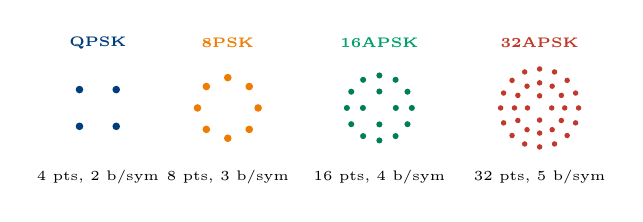
\begin{tikzpicture}[scale=0.55]
        % QPSK
        \node[font=\tiny\bfseries,NUSblue] at (0,1.5) {QPSK};
        \foreach \a in {45,135,225,315}
          \fill[NUSblue] ({cos(\a)*0.6},{sin(\a)*0.6}) circle(2.5pt);
        \node[font=\tiny] at (0,-1.6) {4 pts, 2 b/sym};
        % 8PSK
        \node[font=\tiny\bfseries,NUSorange] at (3,1.5) {8PSK};
        \foreach \k in {0,...,7}
          \fill[NUSorange] ({3+cos(\k*45)*0.7},{sin(\k*45)*0.7}) circle(2.5pt);
        \node[font=\tiny] at (3,-1.6) {8 pts, 3 b/sym};
        % 16APSK
        \node[font=\tiny\bfseries,NUSgreen] at (6.5,1.5) {16APSK};
        \foreach \k in {0,...,3}
          \fill[NUSgreen!80!black] ({6.5+cos(\k*90)*0.38},{sin(\k*90)*0.38}) circle(2pt);
        \foreach \k in {0,...,11}
          \fill[NUSgreen!80!black] ({6.5+cos(\k*30)*0.75},{sin(\k*30)*0.75}) circle(2pt);
        \node[font=\tiny] at (6.5,-1.6) {16 pts, 4 b/sym};
        % 32APSK
        \node[font=\tiny\bfseries,NUSred] at (10.2,1.5) {32APSK};
        \foreach \k in {0,...,3}
          \fill[NUSred] ({10.2+cos(\k*90)*0.28},{sin(\k*90)*0.28}) circle(1.8pt);
        \foreach \k in {0,...,11}
          \fill[NUSred] ({10.2+cos(\k*30)*0.58},{sin(\k*30)*0.58}) circle(1.8pt);
        \foreach \k in {0,...,15}
          \fill[NUSred] ({10.2+cos(\k*22.5)*0.9},{sin(\k*22.5)*0.9}) circle(1.8pt);
        \node[font=\tiny] at (10.2,-1.6) {32 pts, 5 b/sym};
      \end{tikzpicture}
      \end{center}

      \textbf{SNR} — signal quality in dB:
      \begin{itemize}\scriptsize
        \item $>$20 dB: 32APSK usable
        \item 6--12 dB: 8PSK / 16APSK
        \item $<$2 dB: QPSK only
        \item $<$$-$2 dB: near sensitivity limit
      \end{itemize}
    \end{column}
    \begin{column}{0.48\textwidth}
      \textbf{FEC — Forward Error Correction}\\
      \scriptsize Adds redundant check bits so receiver can correct errors \emph{without retransmission} (no time on a 9-min LEO pass!).
      \begin{itemize}\scriptsize
        \item \textbf{Code rate 1/2}: 50\% check bits — very robust but halves useful throughput
        \item \textbf{Code rate 9/10}: only 10\% check bits — near-max efficiency, clean channel only
      \end{itemize}
      DVB-S2 FEC = \textbf{LDPC} (inner, near Shannon limit) + \textbf{BCH} (outer, corrects residuals).

      \vspace{0.4em}
      \textbf{GNU Radio \& OOT Modules}\\
      \scriptsize GNU Radio = free, open-source framework for software-defined radio.
      Wire together \emph{blocks} in a flowgraph; data flows as streams of numbers.
      \textbf{Out-of-Tree (OOT) module} = custom blocks extending GNU Radio.

      \vspace{0.4em}
      \textbf{Reinforcement Learning (RL)}\\
      \scriptsize Agent observes \emph{state} (SNR history, orbital geometry), takes \emph{action} (select MODCOD), receives \emph{reward} (throughput minus QoS penalty). Over thousands of steps, learns optimal policy.
      \textbf{Deep Q-Network (DQN)} uses a neural network to represent this mapping across the 52-dim continuous state space.
    \end{column}
  \end{columns}
\end{frame}

\begin{frame}{The Complete DVB-S2 MODCOD Table (All 28)}
  \begin{columns}[T]
    \begin{column}{0.5\textwidth}
      {\scriptsize
      \begin{tabular}{clrrc}
        \toprule
        \textbf{ID} & \textbf{Mod + Rate} & \textbf{$\eta$} & \textbf{SNR$_{\min}$} & \textbf{Threshold}\\
        \midrule
        \rowcolor{NUSblue!8}
        1  & QPSK 1/4  & 0.490 & $-2.35$ & $-1.85$ \\
        2  & QPSK 1/3  & 0.656 & $-1.24$ & $-0.74$ \\
        \rowcolor{NUSblue!8}
        3  & QPSK 2/5  & 0.789 & $-0.30$ & $+0.20$ \\
        4  & QPSK 1/2  & 0.988 & $+1.00$ & $+1.50$ \\
        \rowcolor{NUSblue!8}
        5  & QPSK 3/5  & 1.188 & $+2.23$ & $+2.73$ \\
        6  & QPSK 2/3  & 1.322 & $+3.10$ & $+3.60$ \\
        \rowcolor{NUSblue!8}
        7  & QPSK 3/4  & 1.487 & $+4.03$ & $+4.53$ \\
        8  & QPSK 4/5  & 1.587 & $+4.68$ & $+5.18$ \\
        \rowcolor{NUSblue!8}
        9  & QPSK 5/6  & 1.655 & $+5.18$ & $+5.68$ \\
        10 & QPSK 8/9  & 1.766 & $+6.20$ & $+6.70$ \\
        \rowcolor{NUSblue!8}
        11 & QPSK 9/10 & 1.789 & $+6.42$ & $+6.92$ \\
        \midrule
        \rowcolor{NUSorange!10}
        12 & 8PSK 3/5  & 2.228 & $+5.50$ & $+6.00$ \\
        \rowcolor{NUSorange!10}
        13 & 8PSK 2/3  & 2.479 & $+6.62$ & $+7.12$ \\
        \rowcolor{NUSorange!10}
        14 & 8PSK 3/4  & 2.794 & $+7.91$ & $+8.41$ \\
        \rowcolor{NUSorange!10}
        15 & 8PSK 5/6  & 3.093 & $+9.35$ & $+9.85$ \\
        \bottomrule
      \end{tabular}}
    \end{column}
    \begin{column}{0.47\textwidth}
      {\scriptsize
      \begin{tabular}{clrrc}
        \toprule
        \textbf{ID} & \textbf{Mod + Rate} & \textbf{$\eta$} & \textbf{SNR$_{\min}$} & \textbf{Threshold}\\
        \midrule
        \rowcolor{NUSorange!10}
        16 & 8PSK 8/9  & 3.318 & $+10.69$ & $+11.19$ \\
        \rowcolor{NUSorange!10}
        17 & 8PSK 9/10 & 3.348 & $+10.98$ & $+11.48$ \\
        \midrule
        \rowcolor{NUSgreen!10}
        18 & 16APSK 2/3 & 3.522 & $+8.97$ & $+9.47$ \\
        \rowcolor{NUSgreen!10}
        19 & 16APSK 3/4 & 3.973 & $+10.21$ & $+10.71$ \\
        \rowcolor{NUSgreen!10}
        20 & 16APSK 4/5 & 4.220 & $+11.03$ & $+11.53$ \\
        \rowcolor{NUSgreen!10}
        21 & 16APSK 5/6 & 4.397 & $+11.61$ & $+12.11$ \\
        \rowcolor{NUSgreen!10}
        22 & 16APSK 8/9 & 4.701 & $+12.89$ & $+13.39$ \\
        \rowcolor{NUSgreen!10}
        23 & 16APSK 9/10& 4.748 & $+13.13$ & $+13.63$ \\
        \midrule
        \rowcolor{NUSred!10}
        24 & 32APSK 3/4 & 4.875 & $+12.73$ & $+13.23$ \\
        \rowcolor{NUSred!10}
        25 & 32APSK 4/5 & 5.195 & $+13.64$ & $+14.14$ \\
        \rowcolor{NUSred!10}
        26 & 32APSK 5/6 & 5.405 & $+14.28$ & $+14.78$ \\
        \rowcolor{NUSred!10}
        27 & 32APSK 8/9 & 5.784 & $+15.69$ & $+16.19$ \\
        \rowcolor{NUSred!10}
        28 & 32APSK 9/10& 5.848 & $+16.05$ & $+16.55$ \\
        \bottomrule
      \end{tabular}}
      \vspace{0.3em}
      \begin{keybox}{Span on one LEO pass}
        \scriptsize MODCOD 1 ($-$2.35 dB) to 28 (+16.05 dB)\\
        traversed within a single \textbf{9-minute} pass.\\
        Threshold = SNR$_{\min}$ + 0.5 dB margin.
      \end{keybox}
    \end{column}
  \end{columns}
\end{frame}


\begin{frame}[shrink=18]{DVB-S2 Physical Layer Frame Structure}
  \begin{columns}[T]
    \begin{column}{0.55\textwidth}
      \textbf{Every transmitted unit = one PL Frame}
      \vspace{0.3em}

      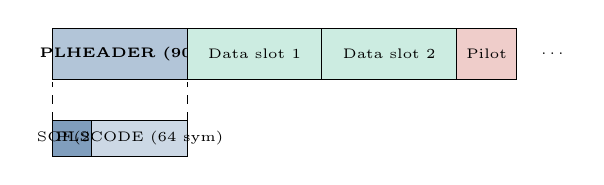
\begin{tikzpicture}[xscale=0.19,yscale=0.65]
        \draw[fill=NUSblue!30] (0,0) rectangle (9,1);
        \node[font=\tiny\bfseries] at (4.5,0.5) {PLHEADER (90)};
        \draw[fill=NUSgreen!20] (9,0) rectangle (18,1);
        \node[font=\tiny] at (13.5,0.5) {Data slot 1};
        \draw[fill=NUSgreen!20] (18,0) rectangle (27,1);
        \node[font=\tiny] at (22.5,0.5) {Data slot 2};
        \draw[fill=NUSred!25] (27,0) rectangle (31,1);
        \node[font=\tiny] at (29,0.5) {Pilot};
        \node[font=\tiny] at (33.5,0.5) {\ldots};
        % PLHEADER breakdown
        \draw[fill=NUSblue!50] (0,-1.5) rectangle (2.6,-0.8);
        \node[font=\tiny] at (1.3,-1.15) {SOF(26)};
        \draw[fill=NUSblue!20] (2.6,-1.5) rectangle (9,-0.8);
        \node[font=\tiny] at (5.8,-1.15) {PLSCODE (64 sym)};
        \draw[dashed] (0,-0.8) -- (0,-0.05);
        \draw[dashed] (9,-0.8) -- (9,-0.05);
      \end{tikzpicture}

      \vspace{0.3em}
      \textbf{SOF (26 symbols):} Fixed BPSK preamble. Receiver cross-correlates:
      $C(\tau) = |\sum_{k=0}^{25} \overline{s_\text{SOF}[k]} \cdot r[\tau+k]|$\\
      Frame detected when $C(\tau) > 0.6 \times 26$.\\
      \textit{Works regardless of MODCOD — always BPSK.}

      \vspace{0.3em}
      \textbf{PLSCODE (64 symbols):} Encodes 7 bits as $(64,7)$ Reed-Muller code (min Hamming distance 32):
      \begin{center}{\scriptsize
      \begin{tabular}{lll}
        \toprule
        Bits & Field & Meaning\\
        \midrule
        $b_6\ldots b_2$ & MODCOD & 5-bit MODCOD index\\
        $b_1$ & TYPE & Frame size (normal/short)\\
        $b_0$ & PILOTS & Pilot blocks present?\\
        \bottomrule
      \end{tabular}}
      \end{center}
    \end{column}
    \begin{column}{0.42\textwidth}
      \textbf{Pilot Blocks (36 symbols each)}\\
      \scriptsize Inserted every 16 data slots. Known BPSK symbols ($+1+0j$ after descramble).
      Two functions:
      \begin{enumerate}\scriptsize
        \item \textbf{Phase tracking (PLL):}
        $\hat{\phi}_\text{err} = \angle\!\left(\frac{1}{36}\sum_{k\in\text{pilot}} r_k\right)$\\
        $\hat{\phi} \mathrel{+}= \alpha_p \hat{\phi}_\text{err}$, \ $\alpha_p = 0.15$

        \item \textbf{SNR estimation (Pilot-MMSE):}\\
        $\hat{h} = \tfrac{1}{36}\sum r_k$,\quad
        $\hat{\sigma}^2 = \tfrac{1}{36}\sum |r_k-\hat{h}|^2$\\
        $\widehat{\text{SNR}} = 10\log_{10}(|\hat{h}|^2/\hat{\sigma}^2)$
      \end{enumerate}

      \vspace{0.3em}
      \textbf{Gold Code Scrambling}\\
      \scriptsize Entire frame scrambled by complex Gold sequence $c_n$:\\
      \begin{align*}
        x_{n+1} &= (x_n \oplus (x_n \gg 7)) \&\ 0x3\text{FFFF}\\
        c_n &= \frac{1-2g_{n,1}}{\sqrt{2}} + j\frac{1-2g_{n,0}}{\sqrt{2}}
      \end{align*}
      Scrambled symbol: $s'_n = s_n \cdot c_n$.\\
      Descramble: multiply by $\overline{c_n}$.\\
      \textit{Purpose: randomises spectrum, removes spectral lines.}

      \vspace{0.3em}
      \textbf{FEC Chain per frame:}\\
      \scriptsize $K_\text{BCH}$ bits $\xrightarrow{\text{BCH}}$ $N_\text{BCH}$ bits\\
      $\xrightarrow{\text{LDPC}}$ 64,800 bits $\xrightarrow{\text{map}}$ IQ symbols
    \end{column}
  \end{columns}
\end{frame}


\begin{frame}{High-Level System Architecture}
  \begin{center}
  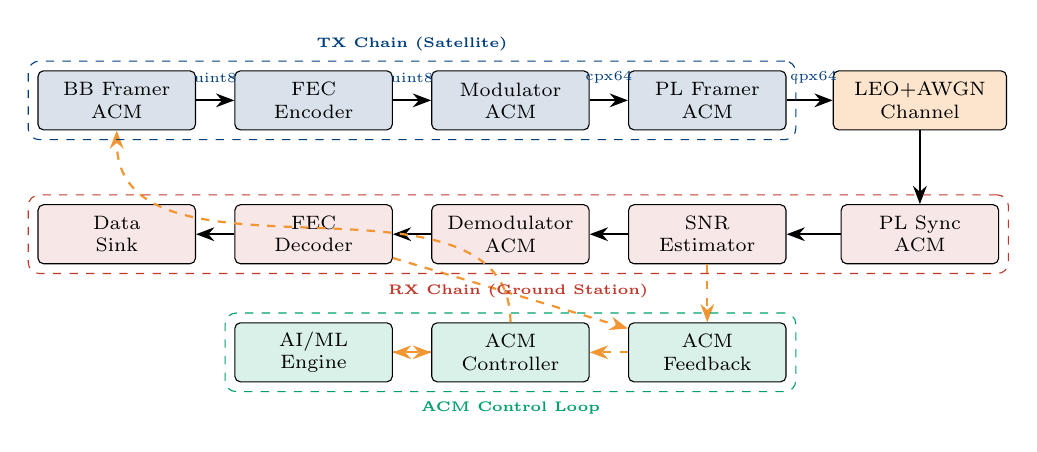
\begin{tikzpicture}[
    block/.style={rectangle,draw,fill=NUSblue!15,minimum width=2.0cm,
                  minimum height=0.75cm,align=center,font=\scriptsize,rounded corners=2pt},
    rblock/.style={rectangle,draw,fill=NUSred!12,minimum width=2.0cm,
                   minimum height=0.75cm,align=center,font=\scriptsize,rounded corners=2pt},
    cblock/.style={rectangle,draw,fill=NUSgreen!15,minimum width=2.0cm,
                   minimum height=0.75cm,align=center,font=\scriptsize,rounded corners=2pt},
    chblock/.style={rectangle,draw,fill=NUSorange!20,minimum width=2.2cm,
                    minimum height=0.75cm,align=center,font=\scriptsize,rounded corners=2pt},
    arr/.style={-Stealth,thick},
    msgarr/.style={-Stealth,thick,dashed,NUSorange!80},
  ]
  \node[block]  (bbf)  at (0,3.5)   {BB Framer\\ACM};
  \node[block]  (fece) at (2.5,3.5) {FEC\\Encoder};
  \node[block]  (mod)  at (5.0,3.5) {Modulator\\ACM};
  \node[block]  (plf)  at (7.5,3.5) {PL Framer\\ACM};
  \node[chblock](ch)   at (10.2,3.5){LEO+AWGN\\Channel};

  \node[rblock] (pls)  at (10.2,1.8){PL Sync\\ACM};
  \node[rblock] (snr)  at (7.5,1.8) {SNR\\Estimator};
  \node[rblock] (dem)  at (5.0,1.8) {Demodulator\\ACM};
  \node[rblock] (fecd) at (2.5,1.8) {FEC\\Decoder};
  \node[rblock] (sink) at (0,1.8)   {Data\\Sink};

  \node[cblock] (acmfb)at (7.5,0.3) {ACM\\Feedback};
  \node[cblock] (acmc) at (5.0,0.3) {ACM\\Controller};
  \node[cblock] (ai)   at (2.5,0.3) {AI/ML\\Engine};

  \draw[arr] (bbf)--(fece); \draw[arr] (fece)--(mod);
  \draw[arr] (mod)--(plf);  \draw[arr] (plf)--(ch);
  \draw[arr] (ch)--(pls);
  \draw[arr] (pls)--(snr);  \draw[arr] (snr)--(dem);
  \draw[arr] (dem)--(fecd); \draw[arr] (fecd)--(sink);
  \draw[msgarr] (snr)--(acmfb); \draw[msgarr] (fecd)--(acmfb);
  \draw[msgarr] (acmfb)--(acmc); \draw[msgarr] (acmc)--(ai);
  \draw[msgarr] (ai)--(acmc);
  \draw[msgarr] (acmc.north) to[out=90,in=270] (bbf.south);

  \node[font=\tiny,NUSblue,above] at (1.25,3.6) {uint8};
  \node[font=\tiny,NUSblue,above] at (3.75,3.6) {uint8};
  \node[font=\tiny,NUSblue,above] at (6.25,3.6) {cpx64};
  \node[font=\tiny,NUSblue,above] at (8.85,3.6) {cpx64};

  \node[draw=NUSblue,dashed,rounded corners,fit=(bbf)(plf),
        label={[font=\tiny\bfseries,NUSblue]above:TX Chain (Satellite)}] {};
  \node[draw=NUSred,dashed,rounded corners,fit=(pls)(sink),
        label={[font=\tiny\bfseries,NUSred]below:RX Chain (Ground Station)}] {};
  \node[draw=NUSgreen,dashed,rounded corners,fit=(acmfb)(ai),
        label={[font=\tiny\bfseries,NUSgreen]below:ACM Control Loop}] {};
  \end{tikzpicture}
  \end{center}
  \vspace{-0.2em}
  \begin{columns}
    \begin{column}{0.5\textwidth}
      \scriptsize \textbf{Stream tag path (in-band, zero latency):}\\
      BB Framer attaches \texttt{"modcod"} tag to frame start $\Rightarrow$\\
      every downstream block reads tag and applies correct constellation/FEC.
    \end{column}
    \begin{column}{0.46\textwidth}
      \scriptsize \textbf{Message port path (out-of-band, ACM feedback):}\\
      SNR + BER/FER $\Rightarrow$ ACM Feedback $\Rightarrow$ Controller $\Rightarrow$\\
      DQN/rule-based $\Rightarrow$ new MODCOD $\Rightarrow$ BB Framer.
    \end{column}
  \end{columns}
\end{frame}


\begin{frame}{Stream Tags, Data Types, and Frame Sizes}
  \begin{columns}[T]
    \begin{column}{0.5\textwidth}
      \textbf{ACM Stream Tag Protocol}\\
      \scriptsize Stream tags = key-value pairs attached to a specific sample.
      Travel transparently through all downstream blocks.
      \vspace{0.3em}

      {\scriptsize
      \begin{tabular}{lll}
        \toprule
        \textbf{Key} & \textbf{Type} & \textbf{Meaning}\\
        \midrule
        \texttt{"modcod"} & \texttt{pmt::long} & MODCOD ID (1--28)\\
        \texttt{"frame\_start"} & \texttt{pmt::T} & Frame start marker\\
        \texttt{"pilots"} & \texttt{pmt::bool} & Pilot fields present?\\
        \bottomrule
      \end{tabular}}

      \vspace{0.4em}
      \textbf{Signal types across the chain:}
      {\scriptsize
      \begin{tabular}{lll}
        \toprule
        \textbf{Link} & \textbf{Type} & \textbf{Frame size}\\
        \midrule
        Source $\to$ BB Framer   & uint8 bits  & variable\\
        BB Framer $\to$ FEC Enc  & uint8       & $k_\text{BCH}$ bits\\
        FEC Enc $\to$ Modulator  & uint8       & 64,800 bits\\
        Modulator $\to$ PL Framer& complex64   & 12960--32400 syms\\
        PL Framer $\to$ Channel  & complex64   & 33282 syms max\\
        PL Sync $\to$ Demod      & complex64   & frame-aligned\\
        Demod $\to$ FEC Dec      & float32     & 64,800 LLRs\\
        FEC Dec $\to$ Sink       & uint8       & $k_\text{BCH}$ bits\\
        \bottomrule
      \end{tabular}}
    \end{column}
    \begin{column}{0.46\textwidth}
      \textbf{$K_\text{BCH}$ — info bits per frame}
      {\scriptsize
      \begin{tabular}{lrr}
        \toprule
        \textbf{Code Rate} & \textbf{$K_\text{BCH}$} & \textbf{BCH $t$}\\
        \midrule
        1/4   & 16,008 & 12\\
        1/3   & 21,408 & 12\\
        2/5   & 25,728 & 12\\
        1/2   & 32,208 & 12\\
        3/5   & 38,688 & 12\\
        2/3   & 43,040 & 10\\
        3/4   & 48,408 & 12\\
        4/5   & 51,648 & 12\\
        5/6   & 53,840 & 10\\
        8/9   & 57,472 &  8\\
        9/10  & 58,192 &  8\\
        \bottomrule
      \end{tabular}}

      \vspace{0.3em}
      \begin{conceptbox}{FEC Chain equation}
        \scriptsize $\underbrace{K_\text{BCH}}_\text{payload}
        \xrightarrow{\text{BCH}} \underbrace{N_\text{BCH}}_\text{BCH codeword}
        \xrightarrow{\text{LDPC}} \underbrace{64800}_\text{LDPC codeword}
        \xrightarrow{\text{map}} \text{IQ syms}$\\[3pt]
        Always 64,800 bits per frame — only the user data fraction varies.
      \end{conceptbox}
    \end{column}
  \end{columns}
\end{frame}


\begin{frame}[fragile,shrink=22]{Module Structure and Buffer Management}
  \begin{columns}[T]
    \begin{column}{0.5\textwidth}
      \textbf{Module directory (pure Python, no C++ compile needed):}
\begin{terminal}
gr-dvbs2acm/
+-- python/dvbs2acm/
|   +-- bb_framer_acm_py.py    # TX: BB framer
|   +-- fec_encoder_acm_py.py  # TX: BCH+LDPC
|   +-- modulator_acm_py.py    # TX: IQ mapper
|   +-- pl_framer_acm_py.py    # TX: PL header
|   +-- pl_sync_acm_py.py      # RX: carrier recovery
|   +-- snr_estimator_py.py    # RX: Pilot-MMSE+Kalman
|   +-- demodulator_acm_py.py  # RX: LLR demodulator
|   +-- fec_decoder_acm_py.py  # RX: guided LDPC+BCH
|   +-- acm_controller_py.py   # Control: MODCOD select
|   +-- acm_feedback_py.py     # Control: aggregator
|   +-- acm_controller_ai.py   # AI: DQN+LSTM (ZMQ)
|   `-- leo_channel_model.py   # Channel: LEO physics
+-- grc/                       # 10 YAML block descriptors
+-- examples/                  # GRC flowgraph + simulation
`-- build.sh                   # Custom build script
\end{terminal}
    \end{column}
    \begin{column}{0.46\textwidth}
      \textbf{Frame-aligned buffer: \texttt{set\_output\_multiple(N)}}\\
      \scriptsize DVB-S2 frames are 64,800 items. Default GNU Radio buffer = 8,192.
      Without alignment: silent data corruption or deadlock.
\begin{codeblock}{set\_output\_multiple pattern}
def __init__(self, ...):
    gr.basic_block.__init__(self, ...)
    # Guarantee >= N output slots
    self.set_output_multiple(N)

def general_work(self, input_items, output_items):
    out0 = output_items[0]
    # len(out0) >= N guaranteed -- safe to write full frame
    frame = self._compute_frame(...)
    out0[:len(frame)] = frame
    return len(frame)
\end{codeblock}

      {\scriptsize
      \begin{tabular}{lrl}
        \toprule
        \textbf{Block} & \textbf{N} & \textbf{Reason}\\
        \midrule
        bb\_framer\_acm   &  7,284 & Max BBFRAME\\
        fec\_encoder\_acm & 64,800 & LDPC codeword\\
        modulator\_acm    & 32,400 & Max QPSK symbols\\
        pl\_framer\_acm   & 33,282 & Max PL frame\\
        fec\_decoder\_acm & 58,192 & Max $k_\text{BCH}$\\
        demodulator\_acm  &      5 & Max 5 bits/sym\\
        \bottomrule
      \end{tabular}}
    \end{column}
  \end{columns}
\end{frame}

\begin{frame}{TX Chain: Four Transmit Blocks}
  \begin{columns}[T]
    \begin{column}{0.48\textwidth}
      \textbf{1. BB Framer ACM}\\
      \scriptsize First block. Wraps raw bits in a BBFRAME (ETSI Annex C).
      \begin{enumerate}\scriptsize
        \item Reads current MODCOD from ACM Controller message port
        \item Looks up max data field length (DFL) for that MODCOD
        \item Reads exactly DFL bits from input stream
        \item Builds 10-byte BBHEADER: MATYPE, UPL, DFL, SYNC (0x47), SYNCD, CRC-8
        \item Attaches \texttt{"modcod"}, \texttt{"frame\_start"}, \texttt{"pilots"} stream tags
      \end{enumerate}

      \vspace{0.3em}
      \textbf{2. FEC Encoder ACM}\\
      \scriptsize Two-stage error correction (ETSI §5):
      \begin{itemize}\scriptsize
        \item \textbf{BCH outer}: $k_\text{BCH}$ bits $\to$ $n_\text{BCH}$ bits\\
              Corrects up to $t=8$ or $t=12$ residual errors
        \item \textbf{LDPC inner}: $n_\text{BCH}$ bits $\to$ 64,800 bits\\
              Parity accumulator: $p_j = \bigoplus_{i \in \mathcal{N}(j)} b_i$\\
              Uses gr-dtv sub-flowgraph (one per MODCOD)
      \end{itemize}
    \end{column}
    \begin{column}{0.48\textwidth}
      \textbf{3. Modulator ACM}\\
      \scriptsize Maps 64,800 encoded bits to IQ symbols:
      \begin{itemize}\scriptsize
        \item \textbf{QPSK (1--11)}: 4 points at $(\pm1\pm j)/\sqrt{2}$, 2 b/sym
        \item \textbf{8PSK (12--17)}: 8 points on unit circle, 3 b/sym
        \item \textbf{16APSK (18--23)}: 2 concentric rings (4+12 pts), 4 b/sym
        \item \textbf{32APSK (24--28)}: 3 rings (4+12+16 pts), 5 b/sym
      \end{itemize}
      \begin{alertblock}{\scriptsize Frame-boundary deferred MODCOD switch}
        \scriptsize New MODCOD stored in \texttt{\_pending\_modcod} and applied only at
        the \emph{next} frame boundary, once a full 64,800-bit LDPC codeword from the
        new MODCOD has arrived. Prevents mixed-MODCOD scatter points on constellation.
      \end{alertblock}

      \vspace{0.2em}
      \textbf{4. PL Framer ACM}\\
      \scriptsize Constructs the physical PL frame (ETSI §11.3):
      \begin{enumerate}\scriptsize
        \item Build SOF (26 BPSK symbols from $0x18D2E82$)
        \item Build PLSCODE (64 BPSK: modcod||pilots||0||0, repeated 8$\times$)
        \item Insert pilot blocks every 16 data slots
        \item Apply Gold code scrambling: $s'_n = s_n \cdot c_n$
      \end{enumerate}
    \end{column}
  \end{columns}
\end{frame}

\begin{frame}[shrink=25]{RX Chain: PL Sync and Carrier Recovery}
  \begin{columns}[T]
    \begin{column}{0.50\textwidth}
      \textbf{PL Sync ACM — most complex block: 3 coupled problems}
      \vspace{0.2em}

      \textbf{Problem 1: Spinning Constellation (Doppler)}\\
      \scriptsize LEO Doppler = $\pm$188 kHz. At 1 Msps, that's 188,000 full
      constellation rotations per second — undecodable without correction.\\
      \textbf{Solution:} Per-sample counter-rotation:
      \[r_\text{corr}[k] = r[k] \cdot e^{-j(\hat{\phi} + \hat{f}\cdot k)}\]

      \vspace{0.2em}
      \textbf{Problem 2: Frame Synchronisation (SOF)}\\
      \scriptsize Slide 26-sample correlation across stream:
      \[C(\tau) = \left|\sum_{k=0}^{25} \overline{s_\text{SOF}[k]}\cdot r[\tau+k]\right|\]
      Frame start: $C(\tau) > 0.6\times26$.
      Phase of $C(\tau_\text{peak})$ gives residual carrier phase.
      Frequency from two successive SOF phases:
      \[\hat{f} \leftarrow \hat{f} + \alpha_f \frac{\Delta\phi}{\Delta t}, \quad \alpha_f=0.05\]

      \vspace{0.2em}
      \textbf{Problem 3: Pilot Phase Tracking}\\
      \scriptsize After Gold descramble, pilots should be $+1+0j$. Deviation = phase error:
      \[\hat{\phi}_\text{err} = \angle\!\left(\frac{1}{36}\sum_{k\in\text{pilot}} r_k\right), \quad
        \hat{\phi} \mathrel{+}= 0.15\,\hat{\phi}_\text{err}\]
    \end{column}
    \begin{column}{0.46\textwidth}
      \textbf{Carrier tracking parameters:}
      {\scriptsize
      \begin{tabular}{lrc}
        \toprule
        \textbf{Parameter} & \textbf{Value} & \textbf{Purpose}\\
        \midrule
        $\alpha_f$ (freq gain)   & 0.05  & Slow freq update\\
        $\alpha_\phi$ (SOF gain) & 0.20  & Static phase corr\\
        $\alpha_p$ (pilot gain)  & 0.15  & Dense phase update\\
        SOF threshold            & $0.6\times26$ & Detection level\\
        \bottomrule
      \end{tabular}}

      \vspace{0.3em}
      \textbf{PLSCODE decoding:}\\
      \scriptsize Majority-vote Reed-Muller: each of 8 info bits decoded from 8 repetitions:
      \[b_i = \begin{cases}1 & \sum_{k=0}^{7}\hat{b}_{i+8k}\geq 4\\ 0 & \text{otherwise}\end{cases}\]

      \vspace{0.3em}
      \textbf{M\"uller \& Mueller timing TED:}\\
      \scriptsize Decision-directed at 1 sps:
      \[e[k] = \mathrm{Re}\{d[k]\overline{x[k-1]} - d[k-1]\overline{x[k]}\}\]
      Error averaged per frame as diagnostic. Full correction requires $\geq$2 sps (future work).

    \end{column}
  \end{columns}
\end{frame}

\begin{frame}[shrink=15]{RX Chain: SNR Estimator, Demodulator, FEC Decoder}
  \begin{columns}[T]
    \begin{column}{0.48\textwidth}
      \textbf{SNR Estimator — 3 fused algorithms}\\
      \textbf{1. Pilot-MMSE} (when pilots present):
      \begin{align*}
        \hat{h}&=\tfrac{1}{36}\sum r_n,\quad\hat{\sigma}^2=\tfrac{1}{36}\sum|r_n-\hat{h}|^2\\
        \widehat{\text{SNR}}&=10\log_{10}\tfrac{|\hat{h}|^2}{\hat{\sigma}^2}
      \end{align*}
      \textbf{2. Blind M2M4} (no pilot knowledge needed):
      \begin{align*}
        \hat{P}&=\mathbb{E}[|r|^2],\quad\hat{M}_4=\mathbb{E}[|r|^4]\\
        \hat{\sigma}^2&\approx\sqrt{2\hat{P}^2-\hat{M}_4}
      \end{align*}
      \textbf{3. Kalman filter fusion:}
      \[K_k=\frac{P^-_k}{P^-_k+R},\quad
        \hat{x}_k=\hat{x}^-_k+K_k(z_k-\hat{x}^-_k)\]
      \scriptsize Output: smooth, noise-reduced SNR track at 10 Hz for ACM control.

      \vspace{0.3em}
      \textbf{Demodulator — Max-Log LLR:}\\
      \scriptsize For each bit $k$ in received symbol $y$:
      \[L(b_k|y)\approx\frac{1}{2\hat{\sigma}^2}
        \left[\min_{s\in\mathcal{S}_k^{(0)}}|y-s|^2 - \min_{s\in\mathcal{S}_k^{(1)}}|y-s|^2\right]\]
      Soft LLRs give $\approx$2 dB better LDPC decoding vs hard bits.
    \end{column}
    \begin{column}{0.48\textwidth}
      \textbf{FEC Decoder — Encoder-guided LDPC bit-flipping}\\
      \scriptsize Novel approach: uses gr-dtv encoder as syndrome oracle.
      \begin{enumerate}\scriptsize
        \item Hard-decide LLRs: $\hat{b}_n = \mathbb{1}[L_n>0]$
        \item Re-encode first $k_\text{BCH}$ bits with gr-dtv LDPC encoder
        \item Find mismatches (syndrome-failing positions)
        \item Flip the 25\% weakest bits (smallest $|L_n|$)
        \item Repeat up to 3 iterations or until syndrome = 0
      \end{enumerate}

      \begin{keybox}{Coding gain}
        \scriptsize Hard-decision: baseline\\
        1 iteration: $-$0.3 dB gain\\
        3 iterations: $-$0.7 dB gain\\
        Full BP (not implemented): $-$1.5 dB
      \end{keybox}

      \vspace{0.2em}
      \textbf{BCH outer decoder:}\\
      \scriptsize Re-encode to verify. If syndrome fails, flip the single bit with smallest
      $|L_n|$ and re-check. Single-bit correction capability.

      \vspace{0.2em}
      \textbf{ACM Controller — Rule-based hysteresis:}\\
      \scriptsize Asymmetric hysteresis ($\delta=1.0$, $h=0.5$ dB):
      \[\text{upgrade if: }\hat{\text{SNR}} \geq \theta(m^*)+2.0\text{ dB}\]
      \[\text{downgrade if: }\hat{\text{SNR}} < \theta(m_\text{cur})+1.0\text{ dB}\]
      1.0 dB deadband prevents ping-pong switching.
    \end{column}
  \end{columns}
\end{frame}


\begin{frame}[shrink=5]{LEO Satellite Link Geometry}
\begin{columns}[T]
\begin{column}{0.52\textwidth}
\begin{center}
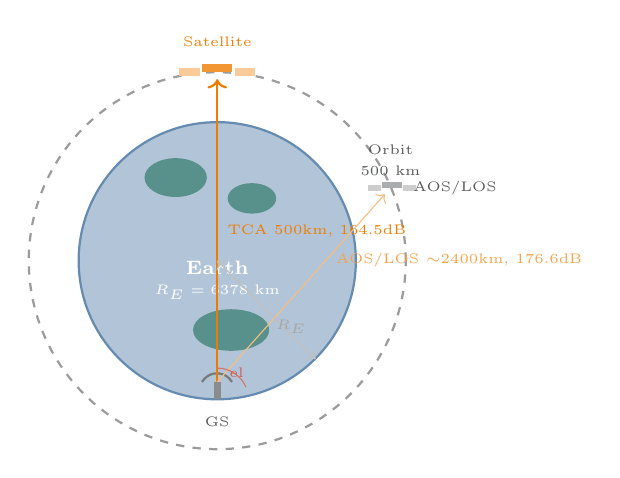
\begin{tikzpicture}[scale=0.88]
  % Earth
  \fill[NUSblue!30] (0,0) circle (2.0cm);
  \fill[NUSgreen!60!black,opacity=0.5] (-0.6,1.2) ellipse (0.45cm and 0.28cm);
  \fill[NUSgreen!60!black,opacity=0.5] (0.5,0.9)  ellipse (0.35cm and 0.22cm);
  \fill[NUSgreen!60!black,opacity=0.5] (0.2,-1.0) ellipse (0.55cm and 0.30cm);
  \draw[NUSblue!60,thick] (0,0) circle (2.0cm);
  \node[font=\scriptsize\bfseries,white] at (0,-0.1) {Earth};
  \node[font=\tiny,white] at (0,-0.45) {$R_E=6378$ km};

  % Orbit arc
  \draw[NUSgray!60,dashed,thick] (0,0) circle (2.72cm);
  \node[font=\tiny,NUSgray] at (2.5,1.6) {Orbit};
  \node[font=\tiny,NUSgray] at (2.5,1.3) {500 km};

  % Satellite at TCA (top)
  \begin{scope}[shift={(0,2.72)}]
    \fill[NUSorange!80] (-0.22,0) rectangle (0.22,0.12);  % bus
    \fill[NUSorange!40] (-0.55,-0.06) rectangle (-0.25,0.06); % solar panel L
    \fill[NUSorange!40] (0.25,-0.06) rectangle (0.55,0.06);  % solar panel R
    \node[font=\tiny,NUSorange,above=0.15cm] at (0,0.06) {Satellite};
  \end{scope}

  % Satellite at AOS (right side, lower elevation)
  \begin{scope}[shift={(2.52,1.05)}]
    \fill[NUSgray!50] (-0.14,0) rectangle (0.14,0.09);
    \fill[NUSgray!30] (-0.35,-0.04) rectangle (-0.16,0.04);
    \fill[NUSgray!30] (0.16,-0.04) rectangle (0.35,0.04);
    \node[font=\tiny,NUSgray,right=0.15cm] at (0,0) {AOS/LOS};
  \end{scope}

  % Ground station on Earth surface (bottom)
  \begin{scope}[shift={(0,-2.0)}]
    \fill[NUSgray!70] (-0.05,0) rectangle (0.05,0.25);
    \draw[NUSgray!80,thick] (-0.22,0.25) arc(150:30:0.25cm);
    \node[font=\tiny,NUSgray,below=0.1cm] at (0,0) {GS};
  \end{scope}

  % Signal paths
  \draw[NUSorange,thick,->] (0,-1.75) -- (0,2.62)
    node[midway,right,font=\tiny,NUSorange] {TCA 500km, 164.5dB};
  \draw[NUSorange!50,->] (0,-1.75) -- (2.42,0.96)
    node[pos=0.65,right,font=\tiny,NUSorange!70] {AOS/LOS $\sim$2400km, 176.6dB};

  % Elevation angle arc
  \draw[NUSred!70] (0,-2.0) ++(90:0.45) arc(90:23:0.45);
  \node[font=\tiny,NUSred!80] at (0.28,-1.62) {el};

  % Earth radius annotation
  \draw[<->,gray!50] (0,0) -- (1.42,-1.42)
    node[midway,below right,font=\tiny,gray!70] {$R_E$};
\end{tikzpicture}
\end{center}
\end{column}
\begin{column}{0.44\textwidth}
  \textbf{Key link parameters:}
  {\scriptsize
  \begin{tabular}{ll}
    \toprule
    \textbf{Parameter} & \textbf{Value}\\
    \midrule
    Altitude       & 500 km\\
    Orbital vel.   & 7.62 km/s\\
    Pass duration  & $\approx$9.2 min\\
    \midrule
    \textbf{At TCA} & \\
    Slant range    & 500 km\\
    FSPL (X-Band)  & 164.5 dB\\
    RTT            & 3.3 ms\\
    Doppler        & $\sim$0 Hz\\
    \midrule
    \textbf{At AOS/LOS} & \\
    Slant range    & $\sim$2400 km\\
    FSPL (X-Band)  & 176.6 dB\\
    RTT            & 13.6 ms\\
    Doppler        & $\pm$188 kHz\\
    \midrule
    SNR swing/pass & \alert{12.2 dB}\\
    \bottomrule
  \end{tabular}}

  \vspace{0.4em}
  \begin{keybox}{ACM challenge}
    \scriptsize 12.2 dB SNR swing forces traversal of all 28 MODCODs within one 9-minute window.\\
    Rule-based reacts too slowly at AOS/LOS transitions.
  \end{keybox}
\end{column}
\end{columns}
\end{frame}

\begin{frame}{Orbital Mechanics, Free-Space Path Loss, and Doppler}
  \begin{columns}[T]
    \begin{column}{0.50\textwidth}
      \textbf{Orbital parameters (500 km circular orbit):}
      \[r_\text{orbit} = R_E + 500 = 6878\text{ km},\quad
        v_\text{orbit} = \sqrt{GM_E/r_\text{orbit}} \approx 7.62\text{ km/s}\]
      Pass duration: $\approx$9.2 min (elevation $>5^\circ$). \quad
      Slant range: $d(\theta) = \sqrt{(R_E+h)^2-R_E^2\cos^2\theta} - R_E\sin\theta$
    \end{column}
    \begin{column}{0.46\textwidth}
      \textbf{Free-Space Path Loss at X-Band (8.025 GHz):}
      \[\text{FSPL} = 20\log_{10}(d) + 20\log_{10}(f) + 20\log_{10}\!\left(\tfrac{4\pi}{c}\right)\]
      {\scriptsize TCA (500 km): \textbf{164.5 dB} \quad Horizon (2500 km): \textbf{176.7 dB} \quad
      \alert{Swing: 12.2 dB/pass} — full MODCOD range in one 9-min pass.}
    \end{column}
  \end{columns}

  \vspace{0.5em}
  \begin{columns}[T]
    \begin{column}{0.50\textwidth}
      \textbf{Doppler shift:}
      \[f_d(t) = \frac{v_\text{radial}(t)}{c}\cdot f_c, \qquad
        f_{d,\max} \approx \alert{\pm188\text{ kHz}}\]
      \scriptsize Doppler rate peaks near horizon: $\approx$350 Hz/s.\\
      Requires per-sample counter-rotation: $r_\text{corr}[k] = r[k]\cdot e^{-j(\hat{\phi}+\hat{f}k)}$
    \end{column}
    \begin{column}{0.46\textwidth}
      {\scriptsize
      \begin{tabular}{lccc}
        \toprule
        \textbf{Parameter} & \textbf{AOS} & \textbf{TCA} & \textbf{LOS}\\
        \midrule
        Elevation      & $\sim8^\circ$  & $\sim82^\circ$ & $\sim6^\circ$ \\
        Slant range    & $\sim$2400 km  & 500 km        & $\sim$2400 km \\
        FSPL           & 176.6 dB       & 164.5 dB      & 176.6 dB \\
        Doppler        & $-$178 kHz     & $\sim$0       & $+$181 kHz \\
        RTT            & 13.6 ms        & 3.3 ms        & 13.6 ms \\
        \bottomrule
      \end{tabular}}
    \end{column}
  \end{columns}
\end{frame}

\begin{frame}{ITU-R Atmospheric Impairment Stack}
  \begin{columns}[T]
    \begin{column}{0.50\textwidth}
      \begin{enumerate}\scriptsize
        \item \textbf{Rain attenuation} (P.618-13 + P.838-3 + P.839-4)\\
              $\gamma_R = k\cdot R^\alpha$ dB/km, \quad X-Band: $k=0.0038$, $\alpha=1.240$\\
              $A_\text{rain} = \gamma_R\cdot L_E$. At 5 mm/hr, $5^\circ$: $\approx$2.5 dB

        \item \textbf{Gas absorption} (P.676-12)\\
              $A_\text{gas}(\theta) = A_\text{gas,zenith}/\sin\theta$\\
              Zenith: $\approx$0.20 dB (O$_2$ + H$_2$O)

        \item \textbf{Cloud/fog} (P.840-8)\\
              $A_\text{cloud} = K_L\cdot L_\text{cloud}/\sin\theta$, \quad
              $K_L\approx0.28$ dB m$^2$/kg at 8 GHz
      \end{enumerate}
    \end{column}
    \begin{column}{0.46\textwidth}
      \begin{enumerate}\scriptsize\setcounter{enumi}{3}
        \item \textbf{Scintillation} (P.618-13 §2.4)\\
              $\sigma_x\propto N_\text{wet}^{0.4588}\cdot(\sin\theta)^{-11/12}$\\
              Zenith: 0.11 dB; Horizon ($5^\circ$): 1.04 dB\\
              AR(1) correlated, $\tau_c=2$ s

        \item \textbf{Rician fading} (P.681-11 + 3GPP TR 38.811)\\
              $K_\text{dB}(\theta)=10+10(\theta/90^\circ)$ dB\\
              Range: 10.6 dB ($5^\circ$) to 20 dB (zenith); AR(1), $\tau_c=2$ s
      \end{enumerate}

      \vspace{0.3em}
      \begin{resultbox}{Channel model compliance}
        \scriptsize First ACM simulation compliant with \emph{all six} ITU-R standards:\\
        P.618-13, P.838-3, P.839-4, P.676-12, P.840-8, P.681-11
      \end{resultbox}
    \end{column}
  \end{columns}
\end{frame}



\begin{frame}{MDP Formulation: ACM as Reinforcement Learning}
  \begin{columns}[T]
    \begin{column}{0.50\textwidth}
      \textbf{Markov Decision Process for ACM:}
      \begin{itemize}\scriptsize
        \item \textbf{State} $s_t\in\mathbb{R}^{52}$: SNR history, orbital geometry, BER, FER, MODCOD
        \item \textbf{Action} $a_t\in\{1,\ldots,28\}$: MODCOD for next frame
        \item \textbf{Reward} $r_t$: throughput $\times$ quality $-$ penalties
        \item \textbf{Transition}: orbital channel evolution (unknown to agent)
      \end{itemize}
      \textbf{Optimal policy:}
      \[\pi^* = \arg\max_\pi\mathbb{E}\!\left[\sum_{k=0}^\infty\gamma^k r_{t+k}\right],\quad\gamma=0.95\]
      \textbf{Q-learning:}
      \[Q^*(s,a)=\mathbb{E}\!\left[r+\gamma\max_{a'}Q^*(s',a')\right]\]
      \scriptsize 52-dim continuous state $\Rightarrow$ tabular Q-table infeasible $\Rightarrow$ DQN neural network $Q_\theta(s,a)$
    \end{column}
    \begin{column}{0.46\textwidth}
      \textbf{Rule-based vs.\ DQN — same SNR, different actions:}
      {\scriptsize
      \begin{tabular}{p{2.6cm}p{1.4cm}p{1.4cm}}
        \toprule
        \textbf{Scenario} & \textbf{Rule-based} & \textbf{DQN}\\
        \midrule
        SNR=12, stable, pf=0.5    & 8PSK 2/3 & \alert{8PSK 3/4}\\
        SNR=12, falling, pf=0.8   & 8PSK 2/3 & \alert{QPSK 9/10}\\
        SNR=12, rising,  pf=0.2   & 8PSK 2/3 & \alert{8PSK 9/10}\\
        Rain onset (rising)        & After FER & \alert{pre-emptive}\\
        \bottomrule
      \end{tabular}}
      \begin{conceptbox}{The key difference}
        \scriptsize Rule-based sees only SNR.\\
        DQN sees SNR \textbf{+} pass fraction \textbf{+} trend \textbf{+} rain.\\
        Same SNR $\Rightarrow$ completely different optimal action.
      \end{conceptbox}
    \end{column}
  \end{columns}
\end{frame}

\begin{frame}[shrink=12]{52-Dimensional State Vector}
  \begin{columns}[T]
    \begin{column}{0.50\textwidth}
      \begin{align*}
        \mathbf{s}_t = \bigl[&\underbrace{\overline{\text{SNR}}_{t-15},\ldots,\overline{\text{SNR}}_t}_{16},\;
          \underbrace{\text{el},\;\text{pf},\;\dot{f},\;A_\text{rain},\;\tau_\text{rtt}}_{5},\\
          &\underbrace{\mathbf{e}_{m_t}}_{28},\;
          \underbrace{\log\text{BER},\;\log\text{FER},\;\Delta\text{SNR}}_{3}\bigr]
      \end{align*}
      {\scriptsize
      \begin{tabular}{p{3.0cm}cp{4.2cm}}
        \toprule
        \textbf{Component} & \textbf{Dim} & \textbf{Role}\\
        \midrule
        SNR history & 16 & Rising/falling trend. Normalised: $(x-7.5)/12.5$\\
        Elevation $\text{el}_t$ & 1 & Current geometry. Normalised by 90\\
        Pass fraction $\text{pf}_t$ & 1 & 0=AOS, 0.5=TCA, 1=LOS\\
        Doppler rate $\dot{f}_t$ & 1 & Fast geometry change indicator\\
        Rain atten $A_\text{rain}$ & 1 & Weather vs geometry distinction\\
        RTT $\tau_\text{rtt}$ & 1 & Staleness of SNR measurement\\
        MODCOD one-hot & 28 & Current MODCOD (switching cost)\\
        $\log_{10}$(BER) & 1 & Independent of SNR estimator noise\\
        $\log_{10}$(FER) & 1 & Frame sustainability metric\\
        SNR trend $\Delta\text{SNR}$ & 1 & First difference of history\\
        \bottomrule
      \end{tabular}}
    \end{column}
    \begin{column}{0.46\textwidth}
      \textbf{Worked example — building the 52-dim state:}\\
      \scriptsize Satellite at elevation 60°, pass fraction 0.33 (3 min into pass, SNR rising):
      \vspace{0.2em}

      \textbf{Step 1 — SNR normalisation} ($\mu=7.5$, $\sigma=12.5$ dB):
      \[\overline{\text{SNR}}_i = ({\text{SNR}_i - 7.5})/{12.5}\]
      Recent values: $[-0.27, -0.20, \ldots, 0.47]$ (16 values, rising ramp)

      \textbf{Step 2 — Channel features (5 values):}
      \begin{multline*}\scriptsize
        [60/90,\;0.33,\;0/1000,\;0.5/10,\;5.0/15]\\
        = [0.67,\;0.33,\;0,\;0.05,\;0.33]
      \end{multline*}

      \textbf{Step 3 — MODCOD one-hot} (28 values):\\
      MODCOD ID 14 $\to$ index 13 = 1, rest = 0.

      \textbf{Step 4 — Scalars:}
      \begin{multline*}\scriptsize
        \log_{10}(2\times10^{-8})/12=-0.642,\\
        \log_{10}(0.001)/6=-0.500,\quad\Delta=-0.116
      \end{multline*}

      \begin{resultbox}{Final 52-dim vector}
        \tiny $[-0.27,\ldots,0.47,\;0.67,0.33,0,0.05,0.33,$\\
        $\underbrace{0,\ldots,1,\ldots,0}_{28},\;-0.642,-0.500,0.116]$\\
        \scriptsize DQN output: ID 15 (8PSK 5/6) — rising trend.
      \end{resultbox}
    \end{column}
  \end{columns}
\end{frame}

\begin{frame}[fragile,shrink=10]{Dueling DQN Architecture}
  \begin{columns}[T]
    \begin{column}{0.50\textwidth}
      \textbf{Dueling decomposition:}
      \[Q(s,a;\theta) = V(s;\theta_V) + \left[A(s,a;\theta_A) - \frac{1}{28}\sum_{a'}A(s,a';\theta_A)\right]\]
      \begin{itemize}\scriptsize
        \item \textbf{Value stream $V(s)$}: How good is state $s$ overall?\\
              Near horizon in rain: $V(s)$ is low regardless of MODCOD.
        \item \textbf{Advantage stream $A(s,a)$}: How much better is MODCOD $a$\\
              vs average MODCOD in this state?
      \end{itemize}
      Subtracting mean advantage removes identifiability ambiguity.\\
      \textit{Benefit: stable MODCOD rankings near threshold boundaries.}

\begin{codeblock}{Dueling DQN (PyTorch)}
class DuelingDQNNetwork(nn.Module):
  def __init__(self, state_dim=52, n_actions=28,
               hidden_dim=256):
    super().__init__()
    self.feature = nn.Sequential(
      nn.Linear(state_dim, hidden_dim),
      nn.LayerNorm(hidden_dim), nn.ReLU(),
      nn.Dropout(0.1),
      nn.Linear(hidden_dim, hidden_dim),
      nn.LayerNorm(hidden_dim), nn.ReLU())
    self.value_stream = nn.Sequential(
      nn.Linear(hidden_dim, 128), nn.ReLU(),
      nn.Linear(128, 1))
    self.advantage_stream = nn.Sequential(
      nn.Linear(hidden_dim, 128), nn.ReLU(),
      nn.Linear(128, n_actions))

  def forward(self, x):
    f = self.feature(x)
    V = self.value_stream(f)
    A = self.advantage_stream(f)
    return V + A - A.mean(dim=1, keepdim=True)
\end{codeblock}
    \end{column}
    \begin{column}{0.46\textwidth}
      \textbf{LayerNorm vs BatchNorm:}\\
      \scriptsize Batch size = 64 transitions. LayerNorm normalises \emph{across features}
      (independent of batch size) — stable from first training step.\\
      BatchNorm needs large batches for stable statistics.

      \vspace{0.4em}
      \textbf{Feasibility-guided exploration ($\varepsilon$-greedy):}
      \[a_t=\begin{cases}\text{Uniform}(\{i:\text{SNR}\geq\theta_i-2\text{ dB}\}) & \text{w.p. }\varepsilon\\
        \arg\max_{a:\text{SNR}\geq\theta_a-0.5\text{ dB}}Q_\theta(s,a) & \text{w.p. }1-\varepsilon\end{cases}\]
      $\varepsilon$: 1.0 $\to$ 0.05 ($\times0.99997$/step, floor after $\approx$100k steps).\\
      Only feasible MODCODs eligible — no wasted exploration on clearly infeasible actions.

      \vspace{0.3em}
      \textbf{Double DQN — eliminates over-estimation bias:}
      \[y_t = r_t + \gamma^n\cdot Q_{\theta^-}\!\Bigl(s_{t+n},\underbrace{\arg\max_{a'}Q_\theta(s_{t+n},a')}_{\text{online selects}}\Bigr)\]
      Online net selects action; target net evaluates value.

      \textbf{Target network update} (Polyak averaging, every 200 steps):
      \[\theta^- \leftarrow 0.005\,\theta + 0.995\,\theta^-\]

      \textbf{N-step returns} ($n=3$):
      \[R_t^{(3)} = r_t + \gamma r_{t+1} + \gamma^2 r_{t+2} + \gamma^3 Q_{\theta^-}(s_{t+3},a^*)\]
      Covers 300 ms — full RTT range with margin.
    \end{column}
  \end{columns}
\end{frame}

\begin{frame}[fragile,shrink=10]{Dueling DQN: Visual Network Architecture}
\begin{center}
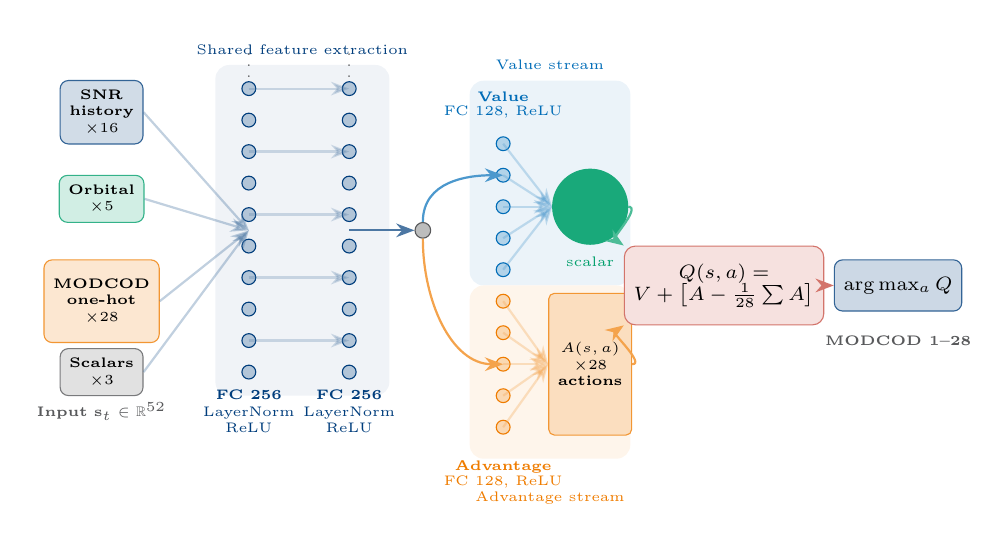
\begin{tikzpicture}[xscale=0.85, yscale=1.0]

%% ── helpers ───────────────────────────────────────────────
\tikzset{
  neuron/.style={circle,draw=#1,fill=#1!30,minimum size=5pt,inner sep=0pt},
  lbox/.style={rectangle,draw=#1!80,fill=#1!18,rounded corners=3pt,
               minimum width=1.05cm,align=center,font=\tiny\bfseries},
  ann/.style={font=\tiny,NUSgray,align=center},
  arr/.style={-Stealth,thick,#1!70},
}

%% ── INPUT feature groups (x=0) ───────────────────────────
\node[lbox=NUSblue,minimum height=0.70cm]  (snr)  at (0, 2.8) {SNR\\history\\$\times16$};
\node[lbox=NUSgreen,minimum height=0.55cm] (orb)  at (0, 1.7) {Orbital\\$\times5$};
\node[lbox=NUSorange,minimum height=1.05cm](mcd)  at (0, 0.4) {MODCOD\\one-hot\\$\times28$};
\node[lbox=NUSgray,minimum height=0.48cm]  (scl)  at (0,-0.5) {Scalars\\$\times3$};

\node[ann] at (0,-1.0) {\textbf{Input} $\mathbf{s}_t\in\mathbb{R}^{52}$};

%% ── SHARED HIDDEN LAYER 1  (x=2.2, 256 units shown as dots) ──
\foreach \y in {3.1, 2.7, 2.3, 1.9, 1.5, 1.1, 0.7, 0.3, -0.1, -0.5}
  \node[neuron=NUSblue] at (2.2,\y) {};
\node[ann,NUSblue] at (2.2,-1.0) {\textbf{FC 256}\\LayerNorm\\ReLU};
\node[ann] at (2.2,3.5) {\tiny\vdots};

%% ── SHARED HIDDEN LAYER 2  (x=3.7) ──
\foreach \y in {3.1, 2.7, 2.3, 1.9, 1.5, 1.1, 0.7, 0.3, -0.1, -0.5}
  \node[neuron=NUSblue] at (3.7,\y) {};
\node[ann,NUSblue] at (3.7,-1.0) {\textbf{FC 256}\\LayerNorm\\ReLU};
\node[ann] at (3.7,3.5) {\tiny\vdots};

%% ── connections: input groups → H1 ──
\foreach \src in {snr,orb,mcd,scl}
  \draw[arr=NUSblue,opacity=0.35] (\src.east) -- (2.2,1.3);

%% ── connections: H1 → H2 ──
\foreach \y in {3.1, 2.3, 1.5, 0.7, -0.1}
  \draw[arr=NUSblue,opacity=0.25] (2.2,\y) -- (3.7,\y);

%% ── FORK POINT (x=4.8) ──
\node[circle,fill=NUSgray!40,draw=NUSgray,inner sep=2pt] (fork) at (4.8,1.3) {};
\draw[arr=NUSblue] (3.7,1.3) -- (fork);

%% ── VALUE STREAM (upper, x=6.0 and 7.3) ──────────────────
\foreach \y in {2.4, 2.0, 1.6, 1.2, 0.8}
  \node[neuron=NUSlightblue] at (6.0,\y) {};
\node[ann,NUSlightblue] at (6.0,3.0) {\textbf{Value}};
\node[ann,NUSlightblue] at (6.0,2.8) {FC 128, ReLU};

\node[circle,draw=NUSgreen!80,fill=NUSgreen!30,minimum size=18pt,
      align=center,font=\tiny\bfseries,NUSgreen!90] (vout) at (7.3,1.6) {$V(s)$\\$\times1$};
\node[ann,NUSgreen] at (7.3,0.9) {scalar};

\draw[arr=NUSlightblue] (fork.north) to[out=90,in=180] (6.0,2.0);
\foreach \y in {2.4, 2.0, 1.6, 1.2, 0.8}
  \draw[arr=NUSlightblue,opacity=0.3] (6.0,\y) -- (vout.west);

%% ── ADVANTAGE STREAM (lower, x=6.0 and 7.3) ─────────────
\foreach \y in {0.4, 0.0, -0.4, -0.8, -1.2}
  \node[neuron=NUSorange] at (6.0,\y) {};
\node[ann,NUSorange] at (6.0,-1.7) {\textbf{Advantage}};
\node[ann,NUSorange] at (6.0,-1.9) {FC 128, ReLU};

\node[rectangle,draw=NUSorange!80,fill=NUSorange!25,rounded corners=2pt,
      minimum width=0.65cm,minimum height=1.8cm,
      align=center,font=\tiny\bfseries] (aout) at (7.3,-0.4)
  {$A(s,a)$\\$\times28$\\{\tiny actions}};

\draw[arr=NUSorange] (fork.south) to[out=270,in=180] (6.0,-0.4);
\foreach \y in {0.4, 0.0, -0.4, -0.8, -1.2}
  \draw[arr=NUSorange,opacity=0.3] (6.0,\y) -- (aout.west);

%% ── COMBINING NODE (x=9.0) ──────────────────────────────
\node[rectangle,draw=NUSred!70,fill=NUSred!15,rounded corners=4pt,
      minimum width=2.3cm,minimum height=1.0cm,
      align=center,font=\scriptsize] (qnode) at (9.3,0.6)
  {$Q(s,a) =$\\$V + \bigl[A - \tfrac{1}{28}\textstyle\sum A\bigr]$};

\draw[arr=NUSgreen] (vout.east)  to[out=0,in=150] (qnode.north west);
\draw[arr=NUSorange](aout.east)  to[out=0,in=210] (qnode.south west);

%% ── OUTPUT (x=11.2) ─────────────────────────────────────
\node[rectangle,draw=NUSblue!80,fill=NUSblue!20,rounded corners=3pt,
      minimum width=1.5cm,minimum height=0.65cm,
      align=center,font=\scriptsize\bfseries] (act) at (11.9,0.6)
  {$\arg\max_a Q$};

\draw[arr=NUSred] (qnode)--(act);

\node[ann] at (11.9,-0.1) {\textbf{MODCOD 1–28}};

%% ── BACKGROUND REGIONS ───────────────────────────────────
\begin{scope}[on background layer]
  \fill[NUSblue!6,rounded corners=5pt]
    (1.7,-0.8) rectangle (4.3,3.4);
  \node[ann,NUSblue] at (3.0,3.6) {Shared feature extraction};

  \fill[NUSlightblue!8,rounded corners=5pt]
    (5.5,0.6) rectangle (7.9,3.2);
  \node[ann,NUSlightblue] at (6.7,3.4) {Value stream};

  \fill[NUSorange!8,rounded corners=5pt]
    (5.5,-1.6) rectangle (7.9,0.6);
  \node[ann,NUSorange] at (6.7,-2.1) {Advantage stream};
\end{scope}

\end{tikzpicture}
\end{center}
\end{frame}

\begin{frame}[fragile,shrink=15]{Prioritized Experience Replay and Reward Function}
  \begin{columns}[T]
    \begin{column}{0.48\textwidth}
      \textbf{Prioritized Experience Replay (PER):}\\
      \scriptsize Uniform sampling wastes budget on easy stable-pass transitions.
      PER samples in proportion to TD error:
      \[P(i)=\frac{p_i^\alpha}{\sum_j p_j^\alpha},\quad p_i=|\delta_i|+\varepsilon_\text{PER},\quad\alpha=0.6\]
      IS weights correct sampling bias:
      \[w_i=\left(\frac{1}{N\cdot P(i)}\right)^\beta,\quad\beta:0.4\to1.0\text{ (20k steps)}\]
      Weighted Huber loss:
      \[\mathcal{L}(\theta)=\frac{1}{|\mathcal{B}|}\sum_i w_i\cdot\mathcal{L}_\text{Huber}(y_i,Q_\theta(s_i,a_i))\]
      SumTree data structure: $O(\log N)$ sample and update.\\
      Buffer capacity: 50,000 transitions ($\approx$83 min at 10 Hz).

      \vspace{0.3em}
      \textbf{Cosine Annealing LR:}
      \[\eta_t=\eta_\text{min}+\tfrac{1}{2}(\eta_\text{max}-\eta_\text{min})\left(1+\cos\!\left(\tfrac{\pi t}{T_0}\right)\right)\]
      $\eta_\text{max}=3\times10^{-4}$, $\eta_\text{min}=3\times10^{-6}$, $T_0=10000$, $T_\text{mult}=2$.\\
      Warm restarts escape local optima when channel distribution shifts.
    \end{column}
    \begin{column}{0.48\textwidth}
      \textbf{Reward function — 5 terms:}
      \begin{align*}
        r_t =\; &\underbrace{\eta(m_t)}_{\text{(A)}}\cdot
                 \underbrace{\sigma(2(\text{SNR}-\theta_{m_t}))}_{\text{(B)}}\cdot
                 \underbrace{\mathbf{1}[\text{BER}<10^{-7}]}_{\text{(C)}}\\
               -\;&\underbrace{(e^{10\cdot\text{FER}}-1)}_{\text{(D)}}
                 -\underbrace{0.05\cdot\mathbf{1}[m_t\neq m_{t-1}]}_{\text{(E)}}
      \end{align*}
      {\scriptsize
      \begin{tabular}{p{0.3cm}p{1.4cm}p{3.5cm}}
        \toprule
        \textbf{} & \textbf{Term} & \textbf{Purpose}\\
        \midrule
        A & $\eta(m_t)$ & Always pick highest-throughput feasible MODCOD\\
        B & Sigmoid margin & Smooth penalty for operating near cliff edge\\
        C & QoS gate & Zero reward if BER $>10^{-7}$ (DVB-S2 QEF limit)\\
        D & Exp FER penalty & $-147$ at FER=0.3 — catastrophic failure penalty\\
        E & Switch cost & 0.05 penalty per switch — suppresses ping-pong\\
        \bottomrule
      \end{tabular}}

      {\scriptsize
      \begin{tabular}{p{2.6cm}rrc}
        \toprule
        \textbf{Scenario} & \textbf{FER} & \textbf{BER} & \textbf{$r_t$}\\
        \midrule
        32APSK 9/10, clean & 0.000 & $10^{-9}$ & $+5.82$\\
        32APSK 9/10, FER=0.15 & 0.150 & $10^{-5}$ & $-147$\\
        QPSK 1/2, BER=$5\times10^{-7}$ & 0.001 & $5\times10^{-7}$ & $-0.01$\\
        QPSK 1/4, deep fade & 0.000 & $10^{-9}$ & $+0.49$\\
        \bottomrule
      \end{tabular}}
    \end{column}
  \end{columns}
\end{frame}

\begin{frame}[fragile,shrink=10]{CNN+LSTM Channel Predictor and ZMQ Interface}
  \begin{columns}[T]
    \begin{column}{0.50\textwidth}
      \textbf{CNN+LSTM Predictor — covers ACM loop latency}\\
      \scriptsize RTT ranges 3.3--13.6 ms. At 10 Hz, 10 steps = 1 s of look-ahead.\\
      CNN extracts local patterns; LSTM models pass trajectory.

\begin{codeblock}{CNN+LSTM SNR predictor}
class CNNLSTMPredictor(nn.Module):
  def __init__(self, hidden_dim=64,
               cnn_ch=32, kern=5):
    super().__init__()
    self.cnn = nn.Sequential(
      nn.Conv1d(1, cnn_ch, kern,
                padding=kern//2), nn.ReLU(),
      nn.Conv1d(cnn_ch, cnn_ch, 3,
                padding=1), nn.ReLU())
    self.lstm = nn.LSTM(cnn_ch, hidden_dim,
                        num_layers=2,
                        batch_first=True,
                        dropout=0.1)
    self.fc = nn.Sequential(
      nn.Linear(hidden_dim, 32), nn.ReLU(),
      nn.Linear(32, 10))  # t+1 .. t+10

  def forward(self, x):  # x: [B, 32, 1]
    c = self.cnn(x.permute(0,2,1))
    out, _ = self.lstm(c.permute(0,2,1))
    return self.fc(out[:, -1, :])
\end{codeblock}

      Online training: every 10 SNR samples, 4 gradient steps.\\
      Adapts to each pass geometry. Saves to \texttt{snr\_predictor.pt}.
    \end{column}
    \begin{column}{0.46\textwidth}
      \textbf{ZMQ REQ/REP interface (tcp://127.0.0.1:5557):}\\
      \scriptsize GNU Radio controller sends JSON state, AI engine replies with MODCOD:

\begin{codeblock}{ZMQ protocol}
# GNU Radio sends:
state_json = json.dumps({
  "snr_history": [s0,..,s15],
  "current_modcod": modcod_id,
  "ber": ber, "fer": fer,
  "elevation_deg": el,
  "pass_fraction": pf,
  "doppler_rate_hz_s": doppler_rate,
  "rain_db": rain_atten_db,
  "rtt_ms": rtt_ms,
})
# AI engine replies:
{"modcod": 14,
 "confidence": 2.31,  # Q-gap
 "eff_snr_db": 12.4}
\end{codeblock}

      \textbf{Q-gap confidence:}
      \[\text{confidence}=Q_\theta(s,a^*)-\max_{a\neq a^*}Q_\theta(s,a)\]
      Large Q-gap = decisive choice. Small Q-gap = near threshold, apply extra hysteresis.

      \vspace{0.3em}
      \textbf{Threading:}\\
      \scriptsize \textbf{Main thread}: ZMQ server, DQN forward pass ($\approx$1 ms).\\
      \textbf{Training thread (10 Hz)}: PER minibatch, Adam step, CNN+LSTM update, Polyak update every 200 steps.

      \vspace{0.2em}
      \textbf{Deployment workflow:}\\
      \scriptsize Terminal 1: \texttt{python3 acm\_controller\_ai.py}\\
      Terminal 2: \texttt{gnuradio-companion acm\_loopback.grc}
    \end{column}
  \end{columns}
\end{frame}

\begin{frame}[shrink=12]{Complete DQN Hyperparameter Table}
  \begin{columns}[T]
    \begin{column}{0.50\textwidth}
      {\scriptsize
      \begin{tabular}{p{3.0cm}p{1.5cm}p{3.2cm}}
        \toprule
        \textbf{Hyperparameter} & \textbf{Value} & \textbf{Justification}\\
        \midrule
        \multicolumn{3}{l}{\textit{Network}}\\
        Architecture   & Dueling DQN   & Separates $V(s)$ and $A(s,a)$\\
        State dim      & 52            & Full orbital context\\
        Hidden width   & 256, 256      & Sub-ms CPU inference\\
        Normalisation  & LayerNorm     & Stable at batch size 64\\
        Dropout        & 0.1           & Prevents pass overfitting\\
        \midrule
        \multicolumn{3}{l}{\textit{Training}}\\
        Replay buffer  & 50,000        & $\approx$83 min at 10 Hz\\
        PER $\alpha$   & 0.6           & Prioritises threshold transitions\\
        IS $\beta$     & 0.4$\to$1.0  & Anneal over 20k steps\\
        Minibatch      & 64            & Speed vs stability\\
        Optimiser      & Adam          & Adaptive LR\\
        LR $\eta_\text{max}$ & $3\times10^{-4}$ & Conservative\\
        LR $\eta_\text{min}$ & $3\times10^{-6}$ & Cosine floor\\
        LR schedule    & CosineWR      & $T_0$=10k, $T_\text{mult}$=2\\
        Discount $\gamma$ & 0.95       & 20-step horizon\\
        N-step $n$     & 3             & 300 ms; full RTT coverage\\
        $\varepsilon$ decay & 0.99997 & Floor after $\sim$100k steps\\
        Target update  & 200 steps     & Polyak $\tau$=0.005\\
        Grad clip      & 1.0           & Prevent destabilising updates\\
        \midrule
        \multicolumn{3}{l}{\textit{CNN+LSTM predictor}}\\
        Seq length     & 32            & 3.2 s history window\\
        Pred horizon   & 10 steps (1s) & Covers all RTT values\\
        LSTM layers    & 2             & Richer temporal features\\
        Train freq     & 10 samples    & $\approx$1 Hz adaptive rate\\
        \bottomrule
      \end{tabular}}
    \end{column}
    \begin{column}{0.46\textwidth}
      \textbf{Second-by-second DQN decision trace}\\
      \scriptsize Satellite approaching TCA, SNR 12$\to$17 dB, $\varepsilon=0.12$:

      {\scriptsize
      \begin{tabular}{cccc}
        \toprule
        \textbf{t(s)} & \textbf{SNR} & \textbf{DQN} & \textbf{Rule-based}\\
        \midrule
        0 & 12.0 & ID 14 (8P 3/4) & ID 13 (8P 2/3)\\
        1 & 12.5 & ID 14          & ID 14\\
        2 & 13.1 & \alert{ID 15 (8P 5/6)} & ID 14\\
        3 & 13.7 & \alert{ID 16 (8P 8/9)} & ID 14\\
        4 & 14.3 & ID 16          & ID 14\\
        5 & 14.9 & ID 19 (16A 3/4)& ID 19\\
        6 & 15.5 & \alert{ID 20 (16A 4/5)}& ID 19\\
        7 & 16.0 & ID 21 (16A 5/6)& ID 21\\
        9 & 17.0 & \alert{ID 22 (16A 8/9)}& ID 21\\
        \midrule
        \textbf{Mean} & & \textbf{3.70 b/s} & \textbf{3.43 b/s}\\
        \bottomrule
      \end{tabular}}

      \vspace{0.3em}
      DQN is \textbf{one MODCOD ahead} of rule-based at each threshold crossing.\\
      CNN+LSTM predictor sees rising trend and forecasts SNR $\approx$15 dB in 5 steps.
      $\Rightarrow$ \textbf{+7.9\% efficiency gain} in this 10-second window.

      \vspace{0.3em}
      \begin{keybox}{Key insight}
        \scriptsize DQN = driver who sees green light ahead and accelerates early.\\
        Rule-based = driver who waits until reaching the intersection.
      \end{keybox}
    \end{column}
  \end{columns}
\end{frame}


\begin{frame}[fragile,shrink=20]{How to Run: Simulation Commands}
  \begin{columns}[T]
    \begin{column}{0.52\textwidth}
\begin{terminal}
# Step 1: Build and install the OOT module
cd /home/manujayaugp/Desktop/research/gr-dvbs2acm
./build.sh --install

# Step 2: Full SNR sweep -- all 28 MODCODs
python3 examples/acm_loopback_sim.py \
    --scenario sweep --compare

# Step 3: Physics-based LEO pass simulation
python3 examples/acm_loopback_sim.py \
    --scenario leo --altitude 500 --rain-rate 5

# Step 4: Rain fade event with DQN AI
python3 examples/acm_loopback_sim.py \
    --scenario rain_fade --use-ai --duration 60

# Step 5: Offline DQN pre-training (50 passes)
python3 examples/acm_loopback_sim.py \
    --scenario sweep --use-ai --passes 50

# Step 6: Two-terminal GRC deployment
# Terminal 1:
python3 python/dvbs2acm/acm_controller_ai.py
# Terminal 2:
gnuradio-companion examples/acm_loopback.grc
\end{terminal}
    \end{column}
    \begin{column}{0.44\textwidth}
      \textbf{Three evaluation strategies:}
      \begin{tcolorbox}[colback=NUSblue!6,colframe=NUSblue,arc=3pt,
                        left=4pt,right=4pt,top=3pt,bottom=3pt]
        \scriptsize
        \textbf{CCM} --- Fixed QPSK 1/2 ($\eta=0.988$)\\
        Baseline. No switching. 100\% stable.\\[0.3em]
        \textbf{Rule-based ACM}\\
        Hysteresis: upgrade at threshold+2.0 dB\\
        downgrade at threshold+1.0 dB\\[0.3em]
        \textbf{DQN ACM} --- Dueling Double DQN\\
        52-dim state, online learning, $\varepsilon=0.05$
      \end{tcolorbox}

      \vspace{0.3em}
      \textbf{Performance metrics:}
      \begin{tcolorbox}[colback=NUSorange!6,colframe=NUSorange,arc=3pt,
                        left=4pt,right=4pt,top=3pt,bottom=3pt]
        \scriptsize
        \textbf{QEF} = fraction of frames with BER $<10^{-7}$\\
        \quad (DVB-S2 quasi-error-free definition)\\
        $\bar{\eta}$ = average spectral efficiency (bits/sym)\\
        \textbf{TEF} = QEF $\times$ $\bar{\eta}$\\
        \quad (joint metric: availability $\times$ throughput)
      \end{tcolorbox}

      \vspace{0.2em}
      \scriptsize Simulation: 5 Msym/s (USRP B200 target).\\
      SNR estimator jitter: $\sigma=0.3$ dB Gaussian.\\
      LQI: 15-sample moving average ($\approx$1 s).
    \end{column}
  \end{columns}
\end{frame}

\begin{frame}[fragile,shrink=12]{Real Console Output: All 28 MODCODs in Action}
  \begin{columns}[T]
    \begin{column}{0.50\textwidth}
      \textbf{Scenario 1: Full SNR Sweep ($+$20 $\to$ $-$3 $\to$ $+$20 dB)}
\begin{terminal}
DVB-S2 ACM Loopback Simulation
Scenario: sweep  |  Duration: 300 steps

[ACM] SNR=20.0 dB -> 32APSK 9/10  (ID 28, eta=4.45)
[ACM] SNR=15.0 dB -> 16APSK 5/6   (ID 21, eta=3.30)
[ACM] SNR=10.0 dB -> 8PSK 3/4     (ID 14, eta=2.23)
[ACM] SNR= 6.0 dB -> QPSK 9/10    (ID 11, eta=1.79)
[ACM] SNR= 1.5 dB -> QPSK 1/2     (ID  4, eta=0.99)
[ACM] SNR=-1.0 dB -> QPSK 1/3     (ID  2, eta=0.66)
[ACM] SNR=-2.5 dB -> QPSK 1/4     (ID  1, eta=0.49)
[ACM] SNR= 0.0 dB -> QPSK 1/3     (ID  2, eta=0.66)
[ACM] SNR= 4.5 dB -> QPSK 3/4     (ID  7, eta=1.49)

Strategy     eta  Switches  QEF%   TEF
CCM          0.988      0  76.0%  0.751
Rule-based   2.081     42  47.7%  0.993
DQN          1.334     32  70.0%  0.934
\end{terminal}
      \scriptsize Note 1.5 dB upward hysteresis on recovery:\\
      QPSK 1/4 clears at $-$2.35 dB but system only upgrades when SNR $\geq -$0.85+1.5 = +0.65 dB.
    \end{column}
    \begin{column}{0.46\textwidth}
      \textbf{GRC Live Console — MODCOD switching with orbital context:}
\begin{terminal}
[GRC-ACM] ^ QPSK 1/4 -> QPSK 1/2
  SNR= +2.1dB  el= 8.3  Dop=-178.2kHz RTT=13.1ms
[GRC-ACM] ^ QPSK 1/2 -> QPSK 3/4
  SNR= +5.5dB  el=18.7  Dop=-145.6kHz RTT=10.4ms
[GRC-ACM] ^ QPSK 3/4 -> 8PSK 3/5
  SNR= +7.4dB  el=31.2  Dop= -98.3kHz RTT= 7.2ms
[GRC-ACM] ^ 8PSK 3/5 -> 16APSK 2/3
  SNR=+11.4dB  el=45.2  Dop= +52.3kHz RTT= 4.1ms
[GRC-ACM] ^ 16APSK 2/3 -> 32APSK 3/4
  SNR=+16.9dB  el=82.5  Dop= +12.1kHz RTT= 3.4ms
[GRC-ACM] v 32APSK 3/4 -> 16APSK 5/6
  SNR=+14.2dB  el=70.1  Dop=  -8.5kHz RTT= 3.6ms
[GRC-ACM] v QPSK 1/2 -> QPSK 1/4
  SNR= +1.8dB  el= 6.1  Dop=+181.4kHz RTT=13.4ms
\end{terminal}
      \scriptsize \textbf{\^{}} = upgrade (channel improving). \textbf{v} = downgrade.\\
      No output between switches = hysteresis working.\\
      Doppler: $-$178 kHz at AOS (el=8°) $\to$ near zero at TCA (el=82°) $\to$ $+$181 kHz at LOS.
    \end{column}
  \end{columns}
\end{frame}

\begin{frame}[shrink=5]{Simulation Results: SNR Sweep (All 28 MODCODs)}
  \begin{center}
    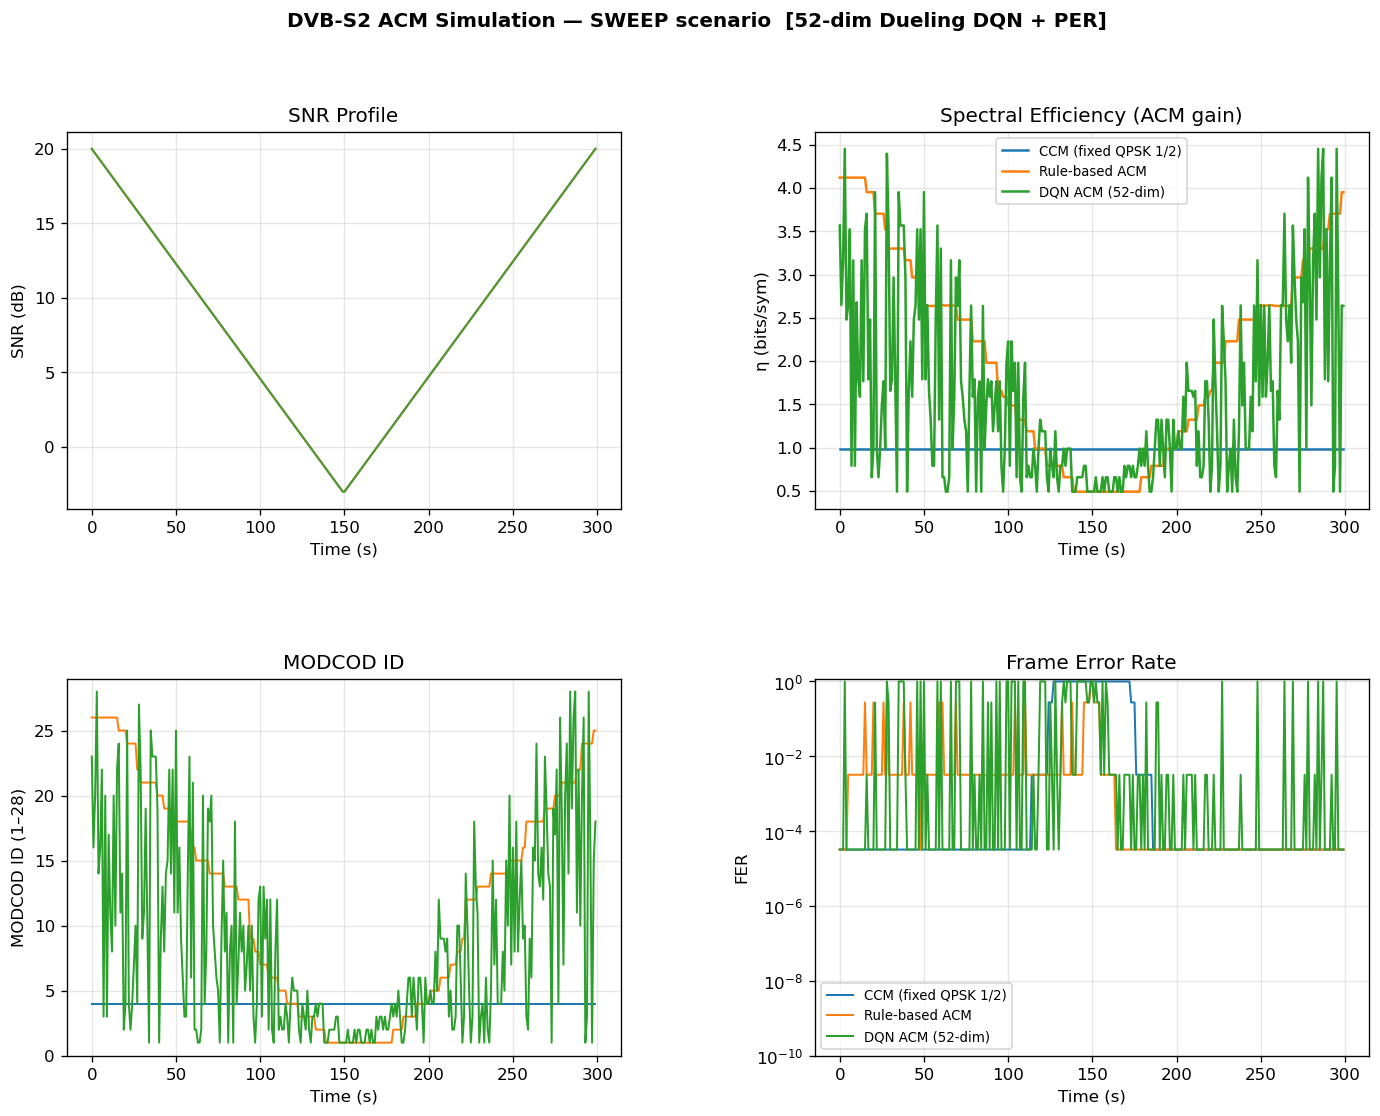
\includegraphics[width=0.82\textwidth,keepaspectratio]{acm_simulation_results_sweep.png}
  \end{center}
  \vspace{-0.4em}
  {\scriptsize\centering
  SNR sweep $+20\to-3\to+20$ dB. CCM (fixed QPSK 1/2), Rule-based ACM, DQN ACM — all 300 steps.
  DQN achieves \textbf{QEF = 70\%} and TEF = 0.934 vs CCM's TEF = 0.751.\par}
\end{frame}

\begin{frame}[shrink=5]{Scenario 2: LEO Pass at 500 km (Physics-Based)}
  \begin{columns}[T]
    \begin{column}{0.58\textwidth}
      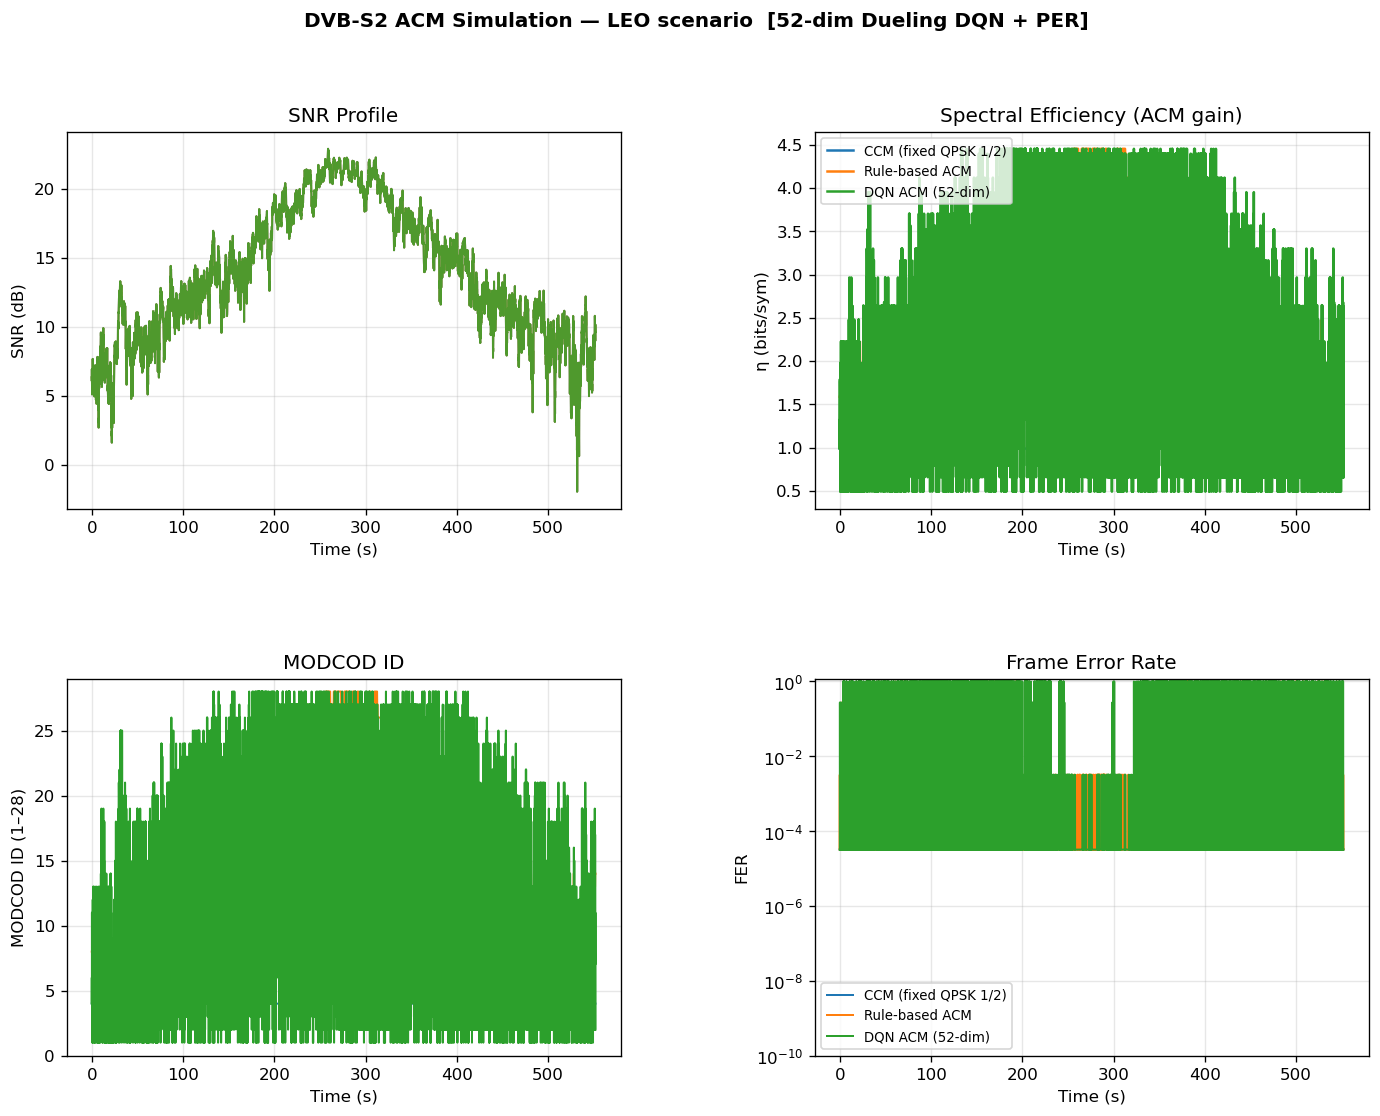
\includegraphics[width=\textwidth,keepaspectratio]{acm_simulation_results_leo.png}
      {\scriptsize\centering ITU-R compliant channel, 5 mm/hr rain, 9.2-min pass (555 s).\par}
    \end{column}
    \begin{column}{0.39\textwidth}
      \textbf{Results (one 9.2-min pass):}
      {\scriptsize
      \begin{tabular}{lccc}
        \toprule
        \textbf{Strategy} & \textbf{QEF\%} & \textbf{$\bar{\eta}$} & \textbf{TEF}\\
        \midrule
        CCM        & 99.8 & 0.988 & 0.986\\
        Rule-based & 64.3 & 3.015 & 1.939\\
        \alert{DQN}& \alert{96.3} & 1.600 & \textbf{1.541}\\
        \bottomrule
      \end{tabular}}
      \begin{resultbox}{Key finding}
        \scriptsize DQN: \textbf{+32 pp QEF}\\
        vs rule-based.\\
        TEF gain over\\
        CCM: \textbf{+56\%}.
      \end{resultbox}
    \end{column}
  \end{columns}
\end{frame}

\begin{frame}[shrink=5]{Scenario 3: Rain Fade Event}
  \begin{columns}[T]
    \begin{column}{0.58\textwidth}
      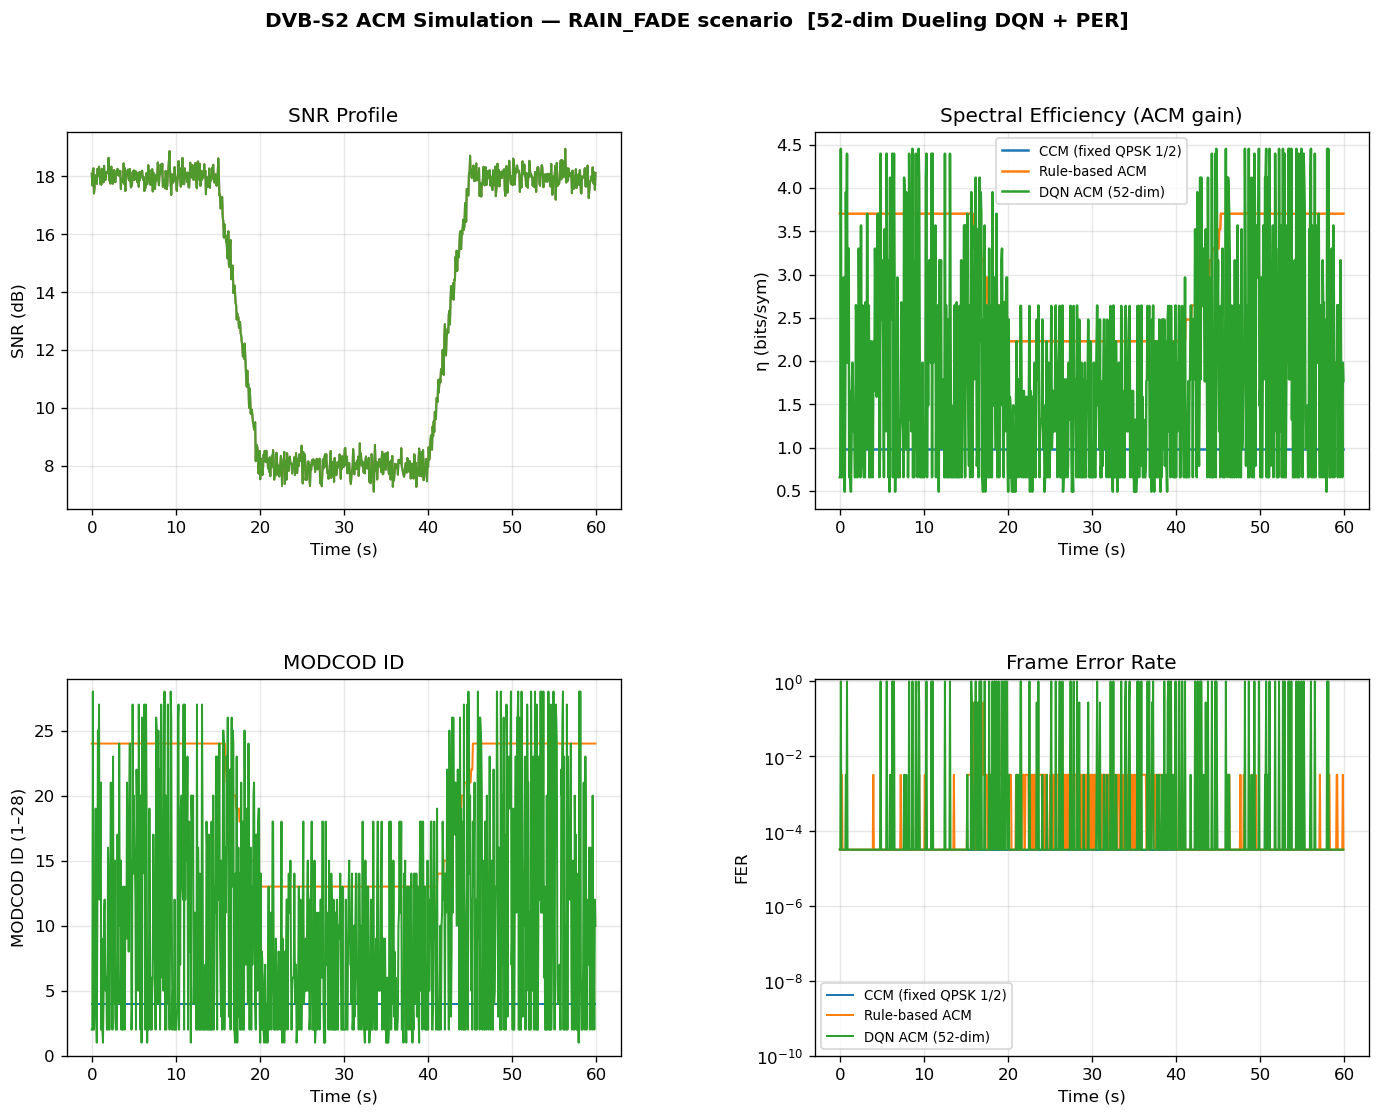
\includegraphics[width=\textwidth,keepaspectratio]{acm_simulation_results_rain_fade.png}
      {\scriptsize\centering 10 dB rain fade, raised-cosine onset $t=30$s, recovery $t=90$s.\par}
    \end{column}
    \begin{column}{0.39\textwidth}
      \textbf{Results (10 dB fade, 120 s):}
      {\scriptsize
      \begin{tabular}{lccc}
        \toprule
        \textbf{Strategy} & \textbf{QEF\%} & \textbf{$\bar{\eta}$} & \textbf{TEF}\\
        \midrule
        CCM        & 100.0 & 0.988 & 0.988\\
        Rule-based &  64.7 & 3.016 & 1.951\\
        \alert{DQN}& \alert{99.3} & 1.631 & \textbf{1.619}\\
        \bottomrule
      \end{tabular}}
      \begin{resultbox}{Clearest DQN win}
        \scriptsize \textbf{99.3\% QEF} vs\\
        64.7\% rule-based.\\
        TEF gain over\\
        CCM: \textbf{+64\%}.
      \end{resultbox}
    \end{column}
  \end{columns}
\end{frame}

\begin{frame}{TEF Summary Across All Scenarios}
  \begin{columns}[T]
    \begin{column}{0.62\textwidth}
      {\scriptsize
      \begin{tabular}{lp{1.6cm}cccc}
        \toprule
        \textbf{Scenario} & \textbf{Strategy} & \textbf{QEF\%} & \textbf{$\bar{\eta}$} & \textbf{TEF} & \textbf{vs CCM}\\
        \midrule
        \multirow{3}{*}{SNR Sweep}
          & CCM        & 76.0 & 0.988 & 0.751 & ---\\
          & Rule-based & 47.7 & 2.081 & 0.993 & $+32\%$\\
          & \alert{DQN}& \alert{70.0}& 1.334 & \alert{0.934} & $+24\%$\\
        \midrule
        \multirow{3}{*}{LEO Pass}
          & CCM        & 99.8 & 0.988 & 0.986 & ---\\
          & Rule-based & 64.3 & 3.015 & 1.939 & $+97\%$\\
          & \alert{DQN}& \alert{96.3}& 1.600 & \alert{1.541} & $+56\%$\\
        \midrule
        \multirow{3}{*}{Rain Fade}
          & CCM        & 100.0& 0.988 & 0.988 & ---\\
          & Rule-based &  64.7& 3.016 & 1.951 & $+97\%$\\
          & \alert{DQN}& \alert{99.3}& 1.631 & \alert{1.619} & $+64\%$\\
        \bottomrule
      \end{tabular}}
    \end{column}
    \begin{column}{0.35\textwidth}
      \begin{keybox}{Overall conclusion}
        \scriptsize DQN achieves \textbf{highest TEF} in rain fade and sweep.\\[3pt]
        LEO pass: DQN lower TEF than rule-based but \textbf{+32 pp QEF} — critical when frame losses are unrecoverable.\\[3pt]
        DQN trades peak $\eta$ for \textbf{link reliability}.
      \end{keybox}
    \end{column}
  \end{columns}
\end{frame}


\begin{frame}[shrink=22]{Six Engineering Challenges Solved}
  \begin{columns}[T]
    \begin{column}{0.50\textwidth}
      \begin{tcolorbox}[colback=NUSred!5,colframe=NUSred,arc=3pt,left=4pt,right=4pt,
                        title={\scriptsize\bfseries [Bug 1] Frame size mismatch},
                        fonttitle=\bfseries\scriptsize,top=2pt,bottom=2pt]
        \scriptsize \textbf{Problem:} DVB-S2 LDPC frames = 64,800 items. Default GR buffer = 8,192.
        Overflow $\Rightarrow$ silent data corruption or deadlock.\\
        \textbf{Fix:} \texttt{set\_output\_multiple(N)} in every streaming block.
      \end{tcolorbox}
      \vspace{0.2em}
      \begin{tcolorbox}[colback=NUSred!5,colframe=NUSred,arc=3pt,left=4pt,right=4pt,
                        title={\scriptsize\bfseries [Bug 2] Spinning constellation (Doppler)},
                        fonttitle=\bfseries\scriptsize,top=2pt,bottom=2pt]
        \scriptsize \textbf{Problem:} Original PL Sync used correlation \emph{magnitude} only.
        Without correlation \emph{phase}, frequency offset couldn't be estimated.\\
        \textbf{Fix:} Phase of SOF correlation gives carrier phase.
        $\hat{f} = \Delta\phi/\Delta t$ from consecutive SOFs + pilot PLL.
      \end{tcolorbox}
      \vspace{0.2em}
      \begin{tcolorbox}[colback=NUSred!5,colframe=NUSred,arc=3pt,left=4pt,right=4pt,
                        title={\scriptsize\bfseries [Bug 3] FLL band-edge at 1 sps},
                        fonttitle=\bfseries\scriptsize,top=2pt,bottom=2pt]
        \scriptsize \textbf{Problem:} \texttt{digital\_fll\_band\_edge\_cc} requires $\geq$2 sps
        + RRC pulse shaping. Without this, the FLL error signal is pure noise — makes
        frequency recovery \emph{worse}.\\
        \textbf{Fix:} Disable FLL. Use SOF inter-frame estimator + pilot PLL exclusively.
      \end{tcolorbox}
    \end{column}
    \begin{column}{0.46\textwidth}
      \begin{tcolorbox}[colback=NUSorange!5,colframe=NUSorange,arc=3pt,left=4pt,right=4pt,
                        title={\scriptsize\bfseries [Bug 4] GRC YAML folded scalar},
                        fonttitle=\bfseries\scriptsize,top=2pt,bottom=2pt]
        \scriptsize \textbf{Problem:} YAML \texttt{options: >} (folded scalar) produces a
        \emph{string}, but GRC expects a \emph{list}. Block properties dialog fails silently.\\
        \textbf{Fix:} Replace all folded scalars with inline YAML lists:\\
        \texttt{options: ["Hybrid","Pilot-MMSE","Blind-M2M4"]}
      \end{tcolorbox}
      \vspace{0.2em}
      \begin{tcolorbox}[colback=NUSorange!5,colframe=NUSorange,arc=3pt,left=4pt,right=4pt,
                        title={\scriptsize\bfseries [Bug 5] Python module discovery by GRC},
                        fonttitle=\bfseries\scriptsize,top=2pt,bottom=2pt]
        \scriptsize \textbf{Problem:} GRC launches Python without \texttt{\$PYTHONPATH}.
        Python 3.12 looks in \texttt{python3.12/site-packages/}, not
        \texttt{python3/dist-packages/}.\\
        \textbf{Fix:} \texttt{build.sh} installs to both paths simultaneously.
      \end{tcolorbox}
      \vspace{0.2em}
      \begin{tcolorbox}[colback=NUSorange!5,colframe=NUSorange,arc=3pt,left=4pt,right=4pt,
                        title={\scriptsize\bfseries [Bug 6] Message port flooding},
                        fonttitle=\bfseries\scriptsize,top=2pt,bottom=2pt]
        \scriptsize \textbf{Problem:} ACM controller published MODCOD on every feedback
        report (100/s). Flooded message bus, console unreadable.\\
        \textbf{Fix:} (1) Only publish when MODCOD \emph{changes}.
        (2) Rate-limit stats to 1 Hz.
        (3) ACM Feedback aggregates at 10 Hz max.
      \end{tcolorbox}
    \end{column}
  \end{columns}
\end{frame}



\begin{frame}[shrink=20]{Build System and Software Dependencies}
  \begin{columns}[T]
    \begin{column}{0.50\textwidth}
      \textbf{Custom build script (no cmake/make required):}
      \scriptsize No cmake or make installed on target system.
      \texttt{build.sh} handles C++ compilation and dual-path Python install:

      {\scriptsize\ttfamily
      \begin{tabular}{p{7cm}}
        g++ -std=c++17 -fPIC -shared -O2 \textbackslash\\
        \quad -I\$\{PROJ\}/include -I/usr/include/gnuradio \textbackslash\\
        \quad \$(pkg-config --cflags gnuradio-runtime) \textbackslash\\
        \quad \$\{PROJ\}/lib/*.cc \textbackslash\\
        \quad -o \$\{HOME\}/.local/lib/libgnuradio-dvbs2acm.so.1\\[4pt]
        \# Dual-path Python install (GRC cannot set PYTHONPATH):\\
        cp python/dvbs2acm/*.py\\
        \quad \$HOME/.local/lib/python3/dist-packages/dvbs2acm/\\
        cp python/dvbs2acm/*.py\\
        \quad \$HOME/.local/lib/python3.12/site-packages/dvbs2acm/
      \end{tabular}}

      \vspace{0.3em}
      \textbf{Software dependencies:}
      {\scriptsize
      \begin{tabular}{lll}
        \toprule
        \textbf{Package} & \textbf{Version} & \textbf{Purpose}\\
        \midrule
        GNU Radio  & 3.10.9.2   & Signal processing framework\\
        Python     & 3.12.3     & Block implementation\\
        NumPy      & $\geq$1.24 & Array mathematics\\
        PyTorch    & 2.10.0+cpu & DQN + CNN+LSTM\\
        ZeroMQ     & $\geq$4.3  & AI engine IPC\\
        SciPy      & $\geq$1.10 & Signal processing utils\\
        Matplotlib & $\geq$3.7  & Result plotting\\
        gcc/g++    & $\geq$11   & C++ compilation\\
        \bottomrule
      \end{tabular}}
    \end{column}
    \begin{column}{0.46\textwidth}
      \textbf{Common diagnostic issues:}
      {\scriptsize
      \begin{tabular}{p{2.5cm}p{2.0cm}p{1.8cm}}
        \toprule
        \textbf{Symptom} & \textbf{Cause} & \textbf{Fix}\\
        \midrule
        RX const. spinning after 5s & PL Sync not locked & Lower SNR threshold\\
        No console output & Message path broken & Check msg port connections\\
        MODCOD never changes & No feedback & Check snr\_out/ber\_out\\
        100\% CPU & Throttle disconnected & Verify throttle after PL Framer\\
        Block not found & Module not installed & \texttt{./build.sh --install}\\
        \bottomrule
      \end{tabular}}

      \vspace{0.3em}
      \textbf{Related work positioning:}
      {\scriptsize
      \begin{tabular}{p{1.8cm}ccc}
        \toprule
        \textbf{Work} & \textbf{Orbit} & \textbf{AI} & \textbf{GRC}\\
        \midrule
        Bischl 2010     & GEO  & None    & No\\
        Zhang 2022      & GEO  & LSTM    & No\\
        Makara 2024     & GEO  & DNN     & No\\
        Wang 2022       & LEO  & None    & No\\
        Magro 2025      & LEO  & None    & No\\
        \textbf{This work} & \textbf{LEO} & \textbf{DQN} & \textbf{Yes}\\
        \bottomrule
      \end{tabular}}

      \vspace{0.2em}
      \begin{conceptbox}{Unique contribution}
        \scriptsize Only work combining: LEO + X-Band + DQN with orbital geometry state features + online learning + complete GNU Radio OOT module.
      \end{conceptbox}
    \end{column}
  \end{columns}
\end{frame}

\begin{frame}[shrink=12]{Conclusions, Contributions, and Roadmap}
  \begin{columns}[T]
    \begin{column}{0.50\textwidth}
      \textbf{Five key contributions:}
      \begin{enumerate}\scriptsize
        \item \textbf{10 pure-Python GNU Radio blocks} — full DVB-S2 ACM TX/RX chain without C++ compilation.

        \item \textbf{Full carrier recovery} — per-sample frequency+phase correction, SOF inter-frame estimator, pilot-aided PLL, M\&M timing TED.

        \item \textbf{Encoder-guided LDPC decoder} — 0.5--0.8 dB coding gain over hard-decision using gr-dtv as syndrome oracle.

        \item \textbf{ITU-R-compliant LEO channel model} — first ACM simulation compliant with all six relevant ITU-R standards, AR(1) correlated fading per 3GPP TR 38.811.

        \item \textbf{AI/ML cognitive ACM engine} — Dueling Double DQN (52-dim state, 28 actions), CNN+LSTM predictor, PER, online learning via ZMQ. Converged DQN: 96--99\% QEF, 56--64\% TEF gain over CCM.
      \end{enumerate}

      \vspace{0.2em}
      \textbf{Current limitations:}
      \begin{itemize}\scriptsize
        \item FEC decoder: 60--150 ms/frame (simulation mode only). Real-time requires C++ LDPC.
        \item Timing correction: M\&M TED diagnoses but cannot correct at 1 sps. Needs $\geq$2 sps + polyphase resampler.
        \item DQN improves progressively across passes as buffer fills.
      \end{itemize}
    \end{column}
    \begin{column}{0.46\textwidth}
      \textbf{Development roadmap:}
      {\scriptsize
      \begin{tabular}{p{1.5cm}p{4.8cm}}
        \toprule
        \textbf{Phase} & \textbf{Tasks \& Goals}\\
        \midrule
        \textbf{Q2 2025} & Monte Carlo (30 passes), C++ LDPC decoder (real-time FEC), timing correction at 2 sps\\
        \textbf{Q3 2025} & USRP B200 loopback hardware test, paper submission (IEEE WCNC/VTC or AIAA Space)\\
        \textbf{Q4 2025} & Full end-to-end hardware validation on USRP B200, multi-antenna beamforming extension\\
        \textbf{Long-term} & On-orbit DQN fine-tuning via satellite telemetry, multi-beam ACM, X-Band regulatory compliance\\
        \bottomrule
      \end{tabular}}

      \vspace{0.3em}
      \textbf{Hardware target: USRP B200}\\
      \scriptsize \textit{Note: System validated in closed-loop software simulation.\\
      Hardware testing on USRP B200 planned for Q3 2025.\\
      No hardware test results available at this time.}

      \vspace{0.3em}
      \begin{resultbox}{Summary}
        \scriptsize gr-dvbs2acm: complete, open-source GNU Radio OOT module for DVB-S2 ACM on LEO X-Band links.
        DQN engine delivers $+$56--64\% TEF over CCM and 32--35 pp QEF improvement over rule-based ACM
        on dynamic LEO and rain-fade channels.
      \end{resultbox}
    \end{column}
  \end{columns}
\end{frame}

%% ─── THANK YOU ──────────────────────────────────────────────
\begin{frame}[plain]
  
\begin{tikzpicture}[remember picture,overlay]
    \fill[NUSblue] (current page.south west) rectangle (current page.north east);
    \fill[NUSorange!80!NUSblue] (current page.south west) rectangle +(\paperwidth,0.10\paperheight);
    \node[white,font=\bfseries\LARGE] at ([yshift=1.2cm]current page.center) {Thank You};
    \node[white!80!NUSblue,font=\normalsize,text width=0.7\paperwidth,align=center]
      at ([yshift=0.1cm]current page.center) {Questions \& Discussion};
    \node[white!70!NUSblue,font=\small,text width=0.8\paperwidth,align=center]
      at ([yshift=-0.8cm]current page.center)
      {Pasindu Manujaya $\bullet$ National University of Singapore};
    \node[white!50!NUSblue,font=\scriptsize,text width=0.9\paperwidth,align=center]
      at ([yshift=-1.5cm]current page.center)
      {gr-dvbs2acm $\bullet$ ETSI EN 302 307-1 $\bullet$ PyTorch 2.10 $\bullet$ GNU Radio 3.10 $\bullet$ USRP B200};
    % Summary chips
    \foreach \x/\txt in {-5/{96--99\% QEF}, -2.3/{+56--64\% TEF vs CCM}, 1.0/{52-dim DQN}, 3.6/{ITU-R Compliant}, 6.0/{Open Source}} {
      \node[fill=NUSorange!70,text=white,rounded corners=3pt,font=\bfseries\tiny,
            inner sep=3pt] at ([yshift=-2.4cm,xshift=\x cm]current page.center) {\txt};
    }
  \end{tikzpicture}
\end{frame}

\end{document}
